%%%%%%%%%%%%%%%%%%%%%%%%%%%%%%%%%%%%%%%%%%%%%%%%%%%%%%%%%%%%%%%%%%%%%%%%%%%%%%%%
%
%  Kafedra ilmiy seminari uchun taqdimot (15 daqiqa, 22 slayd + 1 zaxira slayd)
%  Mavzu: O‘zbek tili gaplarini neyron tarmoqlar asosida sintaktik tahlil
%         qilishning matematik modeli
%  Ixtisoslik: 05.01.07 -- Matematik modellashtirish. Sonli usullar va
%              dasturlar majmui
%  Ma’ruzachi: Matlatipov Sanatbek
%
%  2-tahrir (kafedra seminari fikrlari asosida): graflar nazariyasi atamalari,
%  «hokim» o‘rniga «o‘zak»; boshida korpus, daraxt va semantik ahamiyat misoli;
%  o‘zgartirilgan model (oldin/keyin); ikki optimallashtirish masalasi; MST vaqt
%  tajribasi (n^(n-1) -> O(n^2)); Adam bo‘yicha aniq ishlar va natijalar;
%  «ilk bor» ma’nosidagi ilmiy yangilik.
%
%  Dizayn: HonsAnSkills.tex shabloni (Madrid mavzusi, dolphin rang sxemasi,
%  navigatsiya belgilarisiz), 16:9.  Nutq matni: Matlatipov_seminar_nutq_matni.tex
%
%  Kompilyatsiya:  latexmk -pdf Matlatipov_seminar_taqdimot.tex
%                  (yoki pdflatex ikki marta: kolontitul belgilari uchun)
%
%  Raqamlar manbasi (barchasi repozitoriydagi fayllardan):
%   * validatsiya va o‘qitish egri chiziqlari: saved_models/{pos,depparse}/*_training_log.csv
%     (eng yaxshi nazorat nuqtasi = e’lon qilingan model);
%   * bootstrap: saved_models/depparse/*.dev.pred.conllu (oxirgi qadam bashoratlari);
%   * test va turg‘unlik: paper_materials/review_logs/perturbation_results.json
%     (faqat UAS/LAS), results/spacy_s1.1_test.json;
%   * korpus statistikasi va 2-slayddagi yozuv: data/udbase/*/*.conllu (UzUDT, s658);
%   * parametrlar soni: saved_models/depparse/uz_uzudt_nocharlm_parser.pt (FastText
%     varianti: 24 513 613) va kirish qatlami 500 -> 1143 bo‘yicha hisob (27 563 156);
%     TahrirchiBERT: config.json bo‘yicha 109 486 848;
%   * vaqt tajribasi: mst_vaqt_tajribasi.py -> mst_vaqt_natijalari.json (Apple M2 Max).
%
%%%%%%%%%%%%%%%%%%%%%%%%%%%%%%%%%%%%%%%%%%%%%%%%%%%%%%%%%%%%%%%%%%%%%%%%%%%%%%%%

\documentclass[aspectratio=169,11pt]{beamer}

\usetheme{Madrid}
\usecolortheme{dolphin}
\setbeamertemplate{navigation symbols}{}
\usefonttheme[onlymath]{serif}

\usepackage[utf8]{inputenc}
\usepackage[T1]{fontenc}
\usepackage{lmodern}
\usepackage{amsmath,amssymb,mathtools,bm}
\usepackage{booktabs,multirow,array,tabularx}
\usepackage{fontawesome5}
\usepackage{etoolbox}
\usepackage{appendixnumberbeamer}
\usepackage{tikz}
\usetikzlibrary{arrows.meta,positioning,calc,decorations.pathreplacing,fit,backgrounds,shapes.misc,shapes.geometric,shadows}
\usepackage{pgfplots}
\pgfplotsset{compat=1.18}

\setbeamersize{text margin left=0.7cm,text margin right=0.7cm}
\setbeamerfont{frametitle}{size=\fontsize{11.5}{13.5}\selectfont,series=\bfseries}
\setbeamerfont{block title}{size=\small}
\setbeamerfont{block body}{size=\small}
\setbeamertemplate{blocks}[rounded][shadow=true]

% ---------------------------------------------------------------- ranglar
\definecolor{bmain}{RGB}{51,51,178}        % beamer "structure" rangi
\colorlet{blight}{bmain!10!white}
\colorlet{bsoft}{bmain!35!white}
\definecolor{accent}{RGB}{226,119,32}      % urg‘u (to‘q sariq): men qo‘shgan qismlar
\definecolor{okgreen}{RGB}{38,135,70}
\definecolor{badred}{RGB}{186,48,48}
\definecolor{ftgray}{RGB}{125,125,135}     % FastText seriyasi

% ---------------------------------------------------------------- pgfplots
\pgfplotsset{
  every axis/.append style={
    font=\scriptsize,
    tick label style={font=\tiny},
    label style={font=\scriptsize},
    legend style={font=\tiny,draw=none,fill=white,fill opacity=0.85,text opacity=1},
    axis line style={black!45}, tick style={black!45},
    grid style={black!10}, major grid style={black!10}},
  /pgf/number format/.cd, use comma, 1000 sep={\,},
}

% ---------------------------------------------------------------- TikZ uslublari
\tikzset{
  >={Latex[length=1.8mm]},
  box/.style={rounded corners=3pt,draw=bmain!60,fill=blight,align=center,inner sep=3pt},
  dbox/.style={rounded corners=3pt,fill=bmain,text=white,align=center,inner sep=3pt,font=\bfseries},
  abox/.style={rounded corners=3pt,draw=accent!80,fill=accent!12,align=center,inner sep=3pt},
  stage/.style={rounded corners=3pt,draw=bmain!60,fill=blight,align=center,inner sep=2.5pt,
                font=\scriptsize,minimum height=1.05cm,text width=2.25cm},
  flow/.style={->,thick,bmain!70},
  ref/.style={font=\tiny\itshape,text=black!50},
  % graf chizmalari: uch (so‘z), ildiz, yoy va yoy belgisi
  wn/.style={rounded corners=2pt,draw=bmain!55,fill=blight,font=\scriptsize,inner sep=2pt,minimum height=0.44cm},
  rn/.style={rounded corners=2pt,fill=bmain,text=white,font=\tiny\bfseries,inner sep=2.4pt,minimum height=0.4cm},
  arc/.style={->,thick,bmain!75},
  alab/.style={font=\tiny,fill=white,inner sep=0.6pt,text=bmain!90!black},
}

% ---------------------------------------------------------------- yordamchi buyruqlar
% piktogramma rangli doirada
\newcommand{\ic}[1]{\tikz[baseline=-0.65ex]\node[circle,fill=bmain,text=white,inner sep=0pt,minimum size=0.56cm,font=\footnotesize]{#1};}
% "Ilmiy yangilik N" belgisi: pastki kolontitulning o‘ng qismida
\gdef\yangiliknum{}
\BeforeBeginEnvironment{frame}{\gdef\yangiliknum{}}
\newcommand{\yangilik}[1]{\gdef\yangiliknum{#1}}
\addtobeamertemplate{footline}{}{%
  \ifx\yangiliknum\empty\else
    \begin{tikzpicture}[remember picture,overlay]
      \node[fill=accent,text=white,rounded corners=1.5pt,font=\tiny\bfseries,inner sep=1.4pt]
        at ([xshift=-3.0cm,yshift=0.145cm]current page.south east) {\faLightbulb\ Ilmiy yangilik \yangiliknum};
    \end{tikzpicture}%
  \fi}
% markazlashtirilgan sarlavha qutisi (titul va yakuniy slayd uchun)
\newcommand{\titlebox}[2]{%
  \tikz\node[rounded corners=5pt,fill=bmain!8,draw=bmain!30,text=bmain,align=center,
             text width=#1,inner sep=9pt,drop shadow={opacity=0.25}]{#2};}
% raqamli kartochka (statistik ko‘rsatkich)
\newcommand{\stattile}[3]{%
  \tikz\node[rounded corners=3pt,fill=bmain!10,minimum width=#1,minimum height=0.9cm,align=center,inner sep=2pt]
    {{\color{bmain}\bfseries\small #2}\\[-1pt]{\tiny #3}};}
% to‘q sariq kartochka: men erishgan natija
\newcommand{\mytile}[3]{%
  \tikz\node[rounded corners=3pt,fill=accent!14,draw=accent!60,minimum width=#1,minimum height=0.9cm,align=center,inner sep=2pt]
    {{\color{accent!85!black}\bfseries\small #2}\\[-1pt]{\tiny #3}};}
% ilmiy yangilik kartochkasidagi slayd havolasi
\newcommand{\ysec}[1]{\hfill\mbox{\color{accent}\bfseries\tiny[#1]}}
% manba izohi (alohida xatboshi: ko‘p qatorli izohda qatorlar oralig‘i ham kichik)
\newcommand{\manba}[1]{{\tiny\color{black!55}#1\par}}
% so‘zning tartib raqami (graf uchining indeksi)
\newcommand{\idx}[1]{\textsubscript{\color{black!45}#1}}
% BPE bo‘lagi va oxirgi bo‘lak
\newcommand{\bp}[1]{\tikz[baseline=(b.base)]\node[draw=bmain!45,fill=blight,rounded corners=1.5pt,inner sep=1.6pt,font=\scriptsize\ttfamily](b){\strut #1};}
\newcommand{\bl}[1]{\tikz[baseline=(b.base)]\node[draw=accent,fill=accent!20,rounded corners=1.5pt,inner sep=1.6pt,font=\scriptsize\ttfamily\bfseries](b){\strut #1};}

% o‘zbekcha teorema muhitlari
\newenvironment{tarif}[1][]{\begin{block}{Ta’rif #1}}{\end{block}}
\newenvironment{teorema}[1][]{\begin{block}{Teorema #1}}{\end{block}}
\newenvironment{lemmauz}[1][]{\begin{block}{Lemma #1}}{\end{block}}
\newenvironment{masala}[1][]{\begin{alertblock}{Masala #1}}{\end{alertblock}}
% muallif hissasi bloki (to‘q sariq)
\newenvironment{menblock}[1][\faUserCheck\ Men bajargan ishlar]{%
  \setbeamercolor{block title}{bg=accent,fg=white}%
  \setbeamercolor{block body}{bg=accent!9,fg=black}%
  \begin{block}{#1}}{\end{block}}

\newcommand{\R}{\mathbb{R}}
\DeclareMathOperator*{\argmin}{arg\,min}
\DeclareMathOperator*{\argmax}{arg\,max}
\DeclareMathOperator{\softmax}{softmax}
\DeclareMathOperator{\sgn}{sgn}
\DeclareMathOperator{\ReLU}{ReLU}
\newcommand{\vv}[1]{\mathbf{#1}}
\newcommand{\ind}{\mathbf{1}}

% ---------------------------------------------------------------- titul ma’lumotlari
% !!! Ilmiy rahbar ma’lumotini seminardan oldin tasdiqlang (README.md ga qarang).
\newcommand{\ilmiyrahbar}{f.-m.f.d., professor Aripov Mersaid Mirsidikovich}
\newcommand{\kafedranomi}{Amaliy matematika va kompyuter tahlili kafedrasi}

\title[O‘zbek tili gaplarining sintaktik tahlili]{O‘zbek tili gaplarini neyron tarmoqlar asosida sintaktik tahlil qilishning matematik modeli}
\author[S.~Matlatipov]{Matlatipov Sanatbek}
\institute[O‘zMU]{Mirzo Ulug‘bek nomidagi O‘zbekiston Milliy universiteti}
\date[]{2026}   % qisqa sana bo‘sh: kolontitulda "Ilmiy yangilik" belgisi uchun joy

\begin{document}

%==============================================================================
% 1. TITUL
%==============================================================================
\begin{frame}
  \centering
  \vspace{-6pt}
  \begin{tikzpicture}
    \node[anchor=east] at (0,0) {
\includegraphics[height=1.2cm]{nuu-logo}};
    \node[anchor=west,font=\footnotesize\bfseries,text=bmain] at (0.12,0.2) {MIRZO ULUG‘BEK NOMIDAGI O‘ZBEKISTON MILLIY UNIVERSITETI};
    \node[anchor=west,font=\scriptsize,text=black!70] at (0.12,-0.22) {\kafedranomi};
  \end{tikzpicture}\\[8pt]
  {\normalsize\bfseries MATLATIPOV SANATBEK}\\[8pt]
  \titlebox{0.9\textwidth}{\large\bfseries O‘zbek tili gaplarini neyron tarmoqlar asosida\\ sintaktik tahlil qilishning matematik modeli}\\[9pt]
  {\small 05.01.07 -- Matematik modellashtirish. Sonli usullar va dasturlar majmui}\\[3pt]
  {\small Kafedra ilmiy seminari}\\[10pt]
  {\footnotesize Ilmiy rahbar: \ilmiyrahbar}\\[5pt]
  {\scriptsize\color{black!60} Toshkent -- 2026}
\end{frame}

%==============================================================================
% 2. KORPUSDAN DARAXTGA (yangi)
%==============================================================================
\section{Kirish}
\begin{frame}{Tadqiqot obyekti: korpusdagi yozuv va model chiqishi --- sintaktik daraxt}
  \centering\vspace*{-6pt}
  {\footnotesize\itshape «Bu bo‘limdagi asarlar bizga bu xazinaning eshigini ochib beradi.»}\ \ {\tiny\color{black!55}(UzUDT korpusi, s658-gap)}\\[3pt]
  \begin{tikzpicture}
    % ---------------- chap: korpusdagi CoNLL-U yozuvi
    \node[anchor=north west,font=\scriptsize\bfseries,text=bmain,inner sep=0pt] at (0,0) {\faDatabase\ Korpus: CoNLL-U yozuvi (qo‘lda belgilangan)};
    \node[anchor=north west,draw=bmain!35,fill=bmain!4,rounded corners=2pt,inner sep=3pt] (tbl) at (0,-0.32) {%
      \fontsize{6.6}{7.9}\selectfont\ttfamily
      \setlength{\tabcolsep}{2.6pt}\renewcommand{\arraystretch}{1.03}%
      \begin{tabular}{@{}>{\color{black!55}}r l l l >{\color{accent!85!black}\bfseries}c >{\color{accent!85!black}}l@{}}
        \textbf{ID} & \textbf{FORM} & \textbf{LEMMA} & \textbf{UPOS} & HEAD & \textbf{DEPREL}\\[1pt]
        \hline
        1 & bu & bu & PRON & 2 & det\\
        2 & bo‘limdagi & bo‘lim & ADJ & 3 & amod\\
        3 & asarlar & asar & NOUN & 9 & nsubj\\
        4 & bizga & biz & PRON & 9 & obl\\
        5 & bu & bu & PRON & 6 & det\\
        6 & xazinaning & xazina & NOUN & 7 & nmod:poss\\
        7 & eshigini & eshik & NOUN & 8 & obj\\
        8 & ochib & och & VERB & 9 & xcomp\\
        9 & beradi & ber & VERB & 0 & root\\
        10 & . & . & PUNCT & 9 & punct\\
      \end{tabular}};
    \node[anchor=north west,font=\tiny,text=black!60,text width=5.6cm,inner sep=0pt] at ([yshift=-3pt]tbl.south west)
      {+ XPOS va morfologik belgilar, masalan \texttt{eshigini}: Case=Acc, Person[psor]=3.\\
       \textcolor{accent!85!black}{\textbf{HEAD}} --- so‘zning \textbf{o‘zagi} raqami, \textcolor{accent!85!black}{\textbf{DEPREL}} --- bog‘lanish turi.};
    \node[anchor=north west,rounded corners=3pt,fill=bmain!10,minimum width=1.75cm,minimum height=0.78cm,align=center,inner sep=1pt] at (0,-5.05)
      {{\color{bmain}\bfseries\small 684}\\[-2pt]{\tiny gap}};
    \node[anchor=north west,rounded corners=3pt,fill=bmain!10,minimum width=1.75cm,minimum height=0.78cm,align=center,inner sep=1pt] at (1.87,-5.05)
      {{\color{bmain}\bfseries\small 7\,582}\\[-2pt]{\tiny token}};
    \node[anchor=north west,rounded corners=3pt,fill=bmain!10,minimum width=1.75cm,minimum height=0.78cm,align=center,inner sep=1pt] at (3.74,-5.05)
      {{\color{bmain}\bfseries\small $\kappa\ge0{,}91$}\\[-2pt]{\tiny 6 annotator}};
    % ---------------- o‘rta: model
    \draw[-{Latex[length=3.2mm,width=3.6mm]},line width=3pt,accent] (5.85,-2.35) -- (7.0,-2.35);
    \node[font=\tiny\bfseries,text=accent!85!black,align=center] at (6.42,-1.85) {model};
    \node[font=\tiny,text=black!60,align=center] at (6.42,-2.85) {neyron tarmoq\\+ MST};
    % ---------------- o‘ng: daraxt (graf)
    \node[anchor=north,font=\scriptsize\bfseries,text=bmain,inner sep=0pt] at (10.45,0) {\faSitemap\ Chiqish: yo‘naltirilgan daraxt (graf)};
    \node[rn] (R) at (10.45,-0.62) {ROOT\idx{0}};
    \node[wn] (n9) at (10.45,-1.42) {beradi\idx{9}};
    \node[wn] (n3) at (8.15,-2.37) {asarlar\idx{3}};
    \node[wn] (n4) at (9.65,-2.37) {bizga\idx{4}};
    \node[wn] (n8) at (11.2,-2.37) {ochib\idx{8}};
    \node[wn] (n10) at (12.65,-2.37) {.\idx{10}};
    \node[wn] (n2) at (8.15,-3.27) {bo‘limdagi\idx{2}};
    \node[wn] (n7) at (11.2,-3.27) {eshigini\idx{7}};
    \node[wn] (n1) at (8.15,-4.17) {bu\idx{1}};
    \node[wn] (n6) at (11.2,-4.17) {xazinaning\idx{6}};
    \node[wn] (n5) at (11.2,-5.07) {bu\idx{5}};
    \foreach \a/\b/\l/\p in {R/n9/root/0.5, n9/n3/nsubj/0.62, n9/n4/obl/0.62, n9/n8/xcomp/0.62, n9/n10/punct/0.62,
                             n3/n2/amod/0.5, n2/n1/det/0.5, n8/n7/obj/0.5, n7/n6/nmod:poss/0.5, n6/n5/det/0.5}
      \draw[arc] (\a) -- node[alab,pos=\p] {\l} (\b);
    \node[font=\tiny,text=black!60,align=left,anchor=north west] at (12.0,-3.05)
      {11 ta uch:\\ 10 so‘z + ildiz;\\ 10 ta yoy;\\ har bir so‘zga\\ \textbf{aynan bitta}\\ yoy kiradi};
  \end{tikzpicture}\\[2pt]
  \tikz\node[rounded corners=3pt,fill=bmain!8,draw=bmain!25,text width=0.97\textwidth,align=center,inner sep=3pt,font=\scriptsize]
    {\textbf{Kirish:} so‘zlar ketma-ketligi $x=(w_1,\dots,w_n)$\quad$\Longrightarrow$\quad\textbf{Chiqish:} har bir so‘zning o‘zagi $h_i$ (HEAD) va bog‘lanish turi $r_i$ (DEPREL), ya’ni \textbf{yo‘naltirilgan daraxt}. \ \textbf{Vazifa:} shu daraxtni avtomatik topish.};
\yangilik{1}
\end{frame}

%==============================================================================
% 3. DARAXT NIMA UCHUN KERAK: SEMANTIKA (yangi)
%==============================================================================
\begin{frame}{Sintaktik daraxt nima uchun kerak: gapning ma’nosini ochish}
  \vspace*{-4pt}
  \begin{columns}[T,onlytextwidth]
  \begin{column}{0.335\textwidth}
    \begin{block}{1. Kim? Kimga? Nimani?}
      \centering
      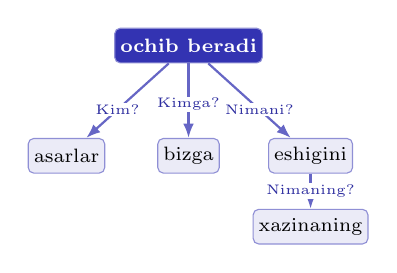
\begin{tikzpicture}[font=\scriptsize]
        \node[wn,fill=bmain,text=white,font=\scriptsize\bfseries] (p) at (0,0) {ochib beradi};
        \node[wn] (a) at (-1.55,-1.4) {asarlar};
        \node[wn] (b) at (0,-1.4) {bizga};
        \node[wn] (c) at (1.55,-1.4) {eshigini};
        \node[wn] (d) at (1.55,-2.3) {xazinaning};
        \draw[arc] (p) -- node[alab,pos=0.62] {Kim?} (a);
        \draw[arc] (p) -- node[alab,pos=0.55] {Kimga?} (b);
        \draw[arc] (p) -- node[alab,pos=0.62] {Nimani?} (c);
        \draw[arc] (c) -- node[alab] {Nimaning?} (d);
      \end{tikzpicture}\\[3pt]
      \raggedright\scriptsize Predikat va uning argumentlari:\\
      \textsc{ochib bermoq}(\textit{kim}: asarlar;\ \textit{kimga}: biz;\ \textit{nimani}: xazina eshigi).
    \end{block}
  \end{column}
  \begin{column}{0.315\textwidth}
    \begin{block}{2. Bir xil so‘zlar --- turli daraxt}
      \centering
      {\scriptsize\itshape «eski kitob do‘koni»}\\[2pt]
      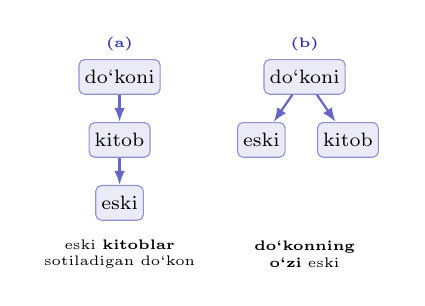
\begin{tikzpicture}[font=\scriptsize]
        \node[font=\tiny\bfseries,text=bmain] at (0,0.42) {(a)};
        \node[wn] (a1) at (0,0) {do‘koni};
        \node[wn] (a2) at (0,-0.8) {kitob};
        \node[wn] (a3) at (0,-1.6) {eski};
        \draw[arc] (a1) -- (a2);
        \draw[arc] (a2) -- (a3);
        \node[font=\tiny\bfseries,text=bmain] at (2.35,0.42) {(b)};
        \node[wn] (b1) at (2.35,0) {do‘koni};
        \node[wn] (b2) at (1.8,-0.8) {eski};
        \node[wn] (b3) at (2.9,-0.8) {kitob};
        \draw[arc] (b1) -- (b2);
        \draw[arc] (b1) -- (b3);
        \node[font=\tiny,align=center,text width=2.1cm] at (0,-2.25) {eski \textbf{kitoblar} sotiladigan do‘kon};
        \node[font=\tiny,align=center,text width=2.1cm] at (2.35,-2.25) {\textbf{do‘konning o‘zi} eski};
      \end{tikzpicture}\\[2pt]
      \scriptsize $\Rightarrow$ \textbf{turli ma’no}
    \end{block}
  \end{column}
  \begin{column}{0.315\textwidth}
    \begin{block}{3. Turli tartib --- bir xil daraxt}
      \centering
      {\scriptsize\itshape «Ali kitobni o‘qidi.» \ $\equiv$\\ «Kitobni Ali o‘qidi.»}\\[3pt]
      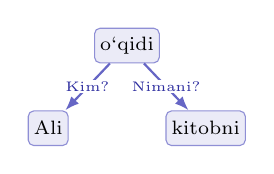
\begin{tikzpicture}[font=\scriptsize]
        \node[wn] (o) at (0,0) {o‘qidi};
        \node[wn] (al) at (-1.0,-1.05) {Ali};
        \node[wn] (k) at (1.0,-1.05) {kitobni};
        \draw[arc] (o) -- node[alab] {Kim?} (al);
        \draw[arc] (o) -- node[alab] {Nimani?} (k);
      \end{tikzpicture}\\[3pt]
      \raggedright\scriptsize $\Rightarrow$ \textbf{bir xil ma’no}: o‘zbek tilida so‘z tartibi erkin, ma’noni qo‘shimchalar va daraxt belgilaydi.
    \end{block}
  \end{column}
  \end{columns}
  \vspace{2pt}
  \begin{alertblock}{\faLightbulb\ Xulosa}
    \scriptsize Gapning ma’nosi so‘zlar ro‘yxatida emas, ular orasidagi \textbf{graf tuzilmasida}. To‘g‘ri daraxt --- \textbf{semantik tahlilning asosi}: mashina tarjimasi (SOV $\to$ SVO tartib), savol-javob tizimlari, matndan axborot ajratish, grammatik tekshiruv.
  \end{alertblock}
\end{frame}

%==============================================================================
% 4. DOLZARBLIK
%==============================================================================
\begin{frame}{Mavzuning dolzarbligi}
\begin{columns}[T,onlytextwidth]
\begin{column}{0.53\textwidth}
  \small
  \begin{tabular}{@{}m{0.7cm}@{}>{\raggedright\arraybackslash}m{6.95cm}@{}}
    \ic{\faLanguage} & O‘zbek tili --- 38 mln dan ortiq kishi so‘zlashadigan \textbf{agglyutinativ} turkiy til. Gapning \textbf{sintaktik tuzilishi} mashina tarjimasi, axborot qidiruvi va savol-javob tizimlari uchun asos.\\ \noalign{\vskip 7pt}
    \ic{\faDatabase} & \textbf{Kam resursli muhit}: Universal Dependencies (UD) tizimida o‘zbek tili uchun bor-yo‘g‘i \textbf{1\,184 ta gap} sintaktik annotatsiyalangan.\\ \noalign{\vskip 7pt}
    \ic{\faCubes} & Kelishik, egalik, son, zamon va shaxs ma’nolari \textbf{qo‘shimchalar zanjiri} bilan ifodalanadi $\Rightarrow$ so‘z shakllari ko‘p, lug‘at siyrak.\\ \noalign{\vskip 7pt}
    \ic{\faProjectDiagram} & Kichik tanlanmada ishonchli ishlaydigan, \textbf{matematik asoslangan} model va \textbf{sonli usullar} (aniq dekodlash, turg‘un o‘qitish) zarur.
  \end{tabular}
\end{column}
\begin{column}{0.44\textwidth}
  \centering
  {\scriptsize\bfseries\color{bmain} So‘z shakli: morfemalar va BPE qism so‘zlari}\\[3pt]
  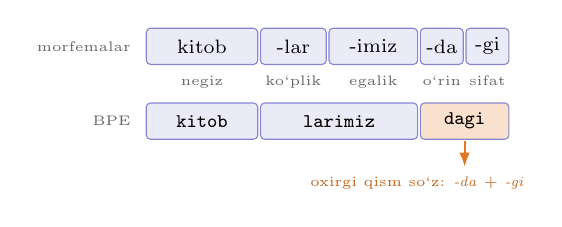
\begin{tikzpicture}[x=0.29cm,y=1cm,font=\scriptsize]
    % morfemalar (1 belgi = 0,29 sm)
    \foreach \a/\b/\t/\g in {0/5/kitob/negiz,5/8/-lar/ko‘plik,8/12/-imiz/egalik,12/14/-da/o‘rin,14/16/-gi/sifat}{
      \draw[rounded corners=1.5pt,draw=bmain!60,fill=blight] (\a+0.06,0) rectangle (\b-0.06,0.46);
      \node at ({(\a+\b)/2},0.23) {\t};
      \node[font=\tiny,text=black!60,anchor=north] at ({(\a+\b)/2},-0.02) {\g};
    }
    \node[anchor=east,font=\tiny,text=black!60] at (-0.2,0.23) {morfemalar};
    % TahrirchiBERT BPE (haqiqiy tokenlash)
    \foreach \a/\b/\t/\c in {0/5/kitob/blight,5/12/larimiz/blight,12/16/dagi/accent!22}{
      \draw[rounded corners=1.5pt,draw=bmain!60,fill=\c] (\a+0.06,-0.95) rectangle (\b-0.06,-0.49);
      \node[font=\scriptsize\ttfamily] at ({(\a+\b)/2},-0.72) {\t};
    }
    \node[anchor=east,font=\tiny,text=black!60] at (-0.2,-0.72) {BPE};
    \draw[->,accent,thick] (14,-0.97) -- (14,-1.3) node[below,font=\tiny,text=accent!85!black,xshift=-0.6cm] {oxirgi qism so‘z: \textit{-da} + \textit{-gi}};
  \end{tikzpicture}\\[6pt]
  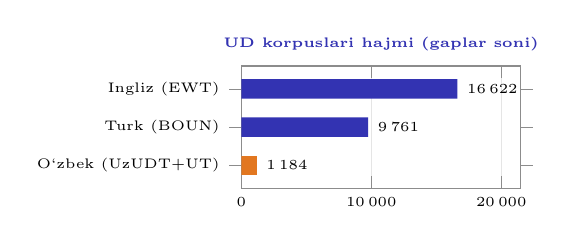
\begin{tikzpicture}
  \begin{axis}[
      scale only axis,width=3.55cm,height=1.55cm,
      xbar,bar width=7pt,
      xmin=0,xmax=21500,
      ymin=0.4,ymax=3.6,
      ytick={1,2,3},
      yticklabels={O‘zbek (UzUDT+UT),Turk (BOUN),Ingliz (EWT)},
      yticklabel style={font=\tiny},
      xtick={0,10000,20000},
      scaled x ticks=false,
      xmajorgrids,
      nodes near coords,
      every node near coord/.append style={font=\tiny},
      title={\tiny\bfseries\color{bmain} UD korpuslari hajmi (gaplar soni)},
      title style={yshift=-4pt},
    ]
    \addplot[fill=accent,draw=none,bar shift=0pt] coordinates {(1184,1)};
    \addplot[fill=bmain,draw=none,bar shift=0pt] coordinates {(9761,2) (16622,3)};
  \end{axis}
  \end{tikzpicture}\\[-1pt]
  \manba{Manba: universaldependencies.org. BPE bo‘linishi --- TahrirchiBERT tokenizatorining haqiqiy natijasi.}
\end{column}
\end{columns}
\end{frame}

%==============================================================================
% 5. O‘RGANILGANLIK DARAJASI
%==============================================================================
\begin{frame}{Muammoning o‘rganilganlik darajasi}
  \centering\vspace*{-6pt}
  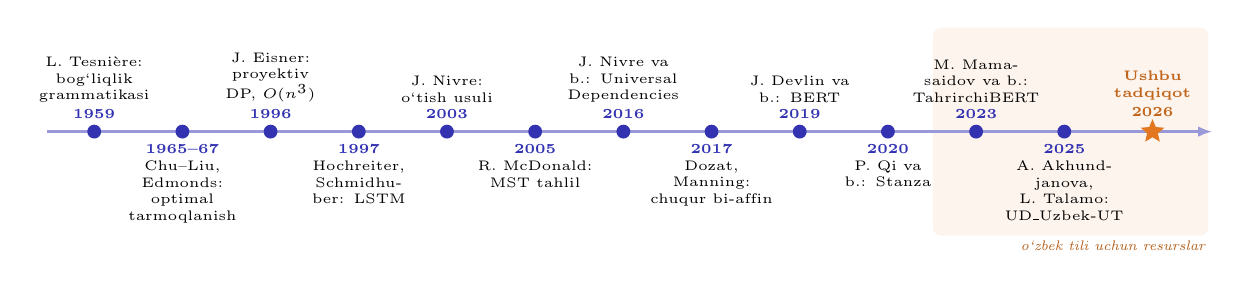
\begin{tikzpicture}[font=\tiny]
    \fill[accent!8,rounded corners=3pt] (10.95,-1.32) rectangle (14.45,1.32);
    \node[font=\tiny\itshape,text=accent!80!black,anchor=north east,inner sep=1pt] at (14.45,-1.34) {o‘zbek tili uchun resurslar};
    \draw[->,bmain!50,line width=1.2pt] (-0.3,0) -- (14.5,0);
    \foreach \x/\yr/\t/\s in {
      0.3/1959/{L.~Tesnière: bog‘liqlik grammatikasi}/1, 1.42/1965--67/{Chu--Liu, Edmonds: optimal tarmoqlanish}/-1,
      2.54/1996/{J.~Eisner: proyektiv DP, $O(n^3)$}/1, 3.66/1997/{Hochreiter, Schmidhuber: LSTM}/-1,
      4.78/2003/{J.~Nivre: o‘tish usuli}/1, 5.9/2005/{R.~McDonald: MST tahlil}/-1,
      7.02/2016/{J.~Nivre va b.: Universal Dependencies}/1, 8.14/2017/{Dozat, Manning: chuqur bi-affin}/-1,
      9.26/2019/{J.~Devlin va b.: BERT}/1, 10.38/2020/{P.~Qi va b.: Stanza}/-1,
      11.5/2023/{M.~Mamasaidov va b.: TahrirchiBERT}/1, 12.62/2025/{A.~Akhundjanova, L.~Talamo: UD\_Uzbek-UT}/-1}{
      \node[circle,fill=bmain,inner sep=0pt,minimum size=5pt] at (\x,0) {};
      \ifnum\s=1
        \node[font=\tiny\bfseries,text=bmain] at (\x,0.22) {\yr};
        \node[text width=1.62cm,align=center,anchor=south,inner sep=1pt] at (\x,0.33) {\t};
      \else
        \node[font=\tiny\bfseries,text=bmain] at (\x,-0.22) {\yr};
        \node[text width=1.62cm,align=center,anchor=north,inner sep=1pt] at (\x,-0.33) {\t};
      \fi
    }
    \node[star,star points=5,star point ratio=2.2,fill=accent,inner sep=0pt,minimum size=9pt] at (13.74,0) {};
    \node[font=\tiny\bfseries,text=accent!85!black] at (13.74,0.25) {2026};
    \node[text width=1.3cm,align=center,font=\tiny\bfseries,text=accent!85!black,anchor=south,inner sep=1pt] at (13.74,0.36) {Ushbu tadqiqot};
  \end{tikzpicture}\\[-2pt]
  \begin{columns}[T,onlytextwidth]
  \begin{column}{0.315\textwidth}
    \begin{block}{\faUniversity\ O‘zbekiston olimlari}
      \scriptsize M.\,M.~Aripov, M.\,X.~Xakimov, G‘.\,R.~Matlatipov, N.~Abdurakhmonova, M.\,S.~Sharipov, E.\,R.~Quriyozov, B.\,B.~Elov, U.\,I.~Salaev, M.~Mamasaidov
    \end{block}
  \end{column}
  \begin{column}{0.315\textwidth}
    \begin{block}{\faGlobe\ Xorijiy va MDH olimlari}
      \scriptsize L.~Tesnière, J.~Edmonds, R.~Tarjan, J.~Eisner, J.~Nivre, R.~McDonald, T.~Dozat, C.\,D.~Manning, P.~Qi, J.~Devlin, M.-C.~de~Marneffe, D.~Zeman, M.~Straka, G.~Eryiğit, U.\,A.~Tukeyev (Qozog‘iston)
    \end{block}
  \end{column}
  \begin{column}{0.315\textwidth}
    \begin{alertblock}{Hal etilmagan masala}
      \scriptsize O‘zbek tili uchun (i) UD sintaktik korpuslari juda kichik va heterogen; (ii) BPE qism so‘zlaridan \textbf{agglyutinativ so‘z vektorini} hosil qilish operatori asoslanmagan; (iii) aniq (MST) va ochko‘z dekodlash hamda modelning \textbf{turg‘unligi} tizimli o‘rganilmagan.
    \end{alertblock}
  \end{column}
  \end{columns}
\end{frame}

%==============================================================================
% 6. MASALANING QO‘YILISHI: GAPNING GRAF MODELI
%==============================================================================
\begin{frame}{Masalaning qo‘yilishi: gapning graf modeli}
\begin{columns}[T,onlytextwidth]
\begin{column}{0.35\textwidth}
  \centering
  {\scriptsize\bfseries\color{bmain} «Ali kitobni o‘qidi» gapining grafi $G_x$}\\[2pt]
  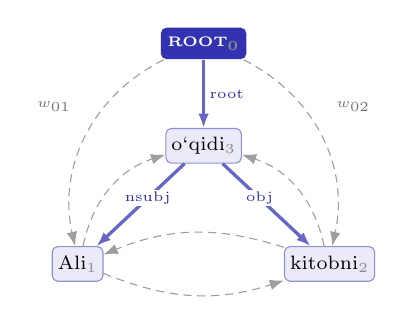
\begin{tikzpicture}[font=\scriptsize]
    \node[rn] (R) at (1.9,2.4) {ROOT\idx{0}};
    \node[wn] (O) at (1.9,1.1) {o‘qidi\idx{3}};
    \node[wn] (A) at (0.3,-0.4) {Ali\idx{1}};
    \node[wn] (K) at (3.5,-0.4) {kitobni\idx{2}};
    % daraxtga kirmagan yoylar
    \begin{scope}[->,black!38,densely dashed]
      \draw (R) to[bend right=38] (A);
      \draw (R) to[bend left=38] (K);
      \draw (A) to[bend left=30] (O);
      \draw (K) to[bend right=30] (O);
      \draw (A) to[bend right=20] (K);
      \draw (K) to[bend right=20] (A);
    \end{scope}
    % qamrovchi daraxt yoylari
    \draw[arc,line width=1.2pt] (R) -- node[alab,right=1pt] {root} (O);
    \draw[arc,line width=1.2pt] (O) -- node[alab,pos=0.42] {nsubj} (A);
    \draw[arc,line width=1.2pt] (O) -- node[alab,pos=0.42] {obj} (K);
    \node[font=\tiny\itshape,text=black!55] at (0.0,1.6) {$w_{01}$};
    \node[font=\tiny\itshape,text=black!55] at (3.8,1.6) {$w_{02}$};
  \end{tikzpicture}\\[3pt]
  \raggedright\scriptsize
  $n=3$: \ $|A|=n^2=9$ ta yoy (shtrix),\\
  qalin --- bitta qamrovchi daraxt;\\
  jami $|\mathcal T(x)|=3^{2}=9$ ta daraxt.\\[4pt]
  \manba{Yoy $j\to i$: $j$ --- \textbf{o‘zak uch}, $i$ --- \textbf{tobe uch}; har bir yoyga vazn $w_{ji}$ beriladi.}
\end{column}
\begin{column}{0.62\textwidth}
  \begin{tarif}[1 (gap grafi va bog‘liqlik daraxti)]
    \scriptsize $x=(w_1,\dots,w_n)$ --- gap; \ $G_x=(V,A,W)$ --- vaznli to‘liq yo‘naltirilgan graf: $V=\{0,1,\dots,n\}$ ($0$ --- ildiz), \ $A=\{j\to i:\ i\ge1,\ j\ne i\}$, $|A|=n^2$; \ $W=(w_{ji})$ --- vazn matritsasi.\\[2pt]
    \textbf{Bog‘liqlik daraxti} $y\subset A$ --- $0$ ildizli \textbf{yo‘naltirilgan qamrovchi daraxt} (arborestsensiya): har bir $i\ge1$ uchun kirish darajasi $\deg^-(i)=1$ (yagona \textbf{o‘zak} $h_i$), sikl yo‘q, $\deg^+(0)=1$; yoy belgisi $r_i\in\mathcal R$, $|\mathcal R|=39$.
  \end{tarif}
  \begin{lemmauz}[1 (A.~Cayley formulasi asosida)]
    \scriptsize $|\mathcal T(x)|=n^{\,n-1}$:\ \ $n=10\Rightarrow10^{9}$;\ \ $\bar n=11{,}4\Rightarrow\approx10^{11}$. \ {\tiny\itshape ($n\le7$ da barcha daraxtlarni sanab tekshirdim.)}
  \end{lemmauz}
  \begin{masala}[(P): eng og‘ir qamrovchi daraxtni topish]
    \scriptsize $\hat y=\argmax\nolimits_{y\in\mathcal T(x)}W(y)$,\ \ $W(y)=\sum\nolimits_{(j\to i)\in y}w_{ji}$,\ \ $w_{ji}=\log P_\theta(h_i=j\mid x)$.\\[1pt]
    Sifat: \ $\mathrm{UAS}=\frac1N\sum_{i}\ind[\hat h_i=h_i]$,\ \ $\mathrm{LAS}=\frac1N\sum_i\ind[\hat h_i=h_i\wedge\hat r_i=r_i]$.
  \end{masala}
\end{column}
\end{columns}
\end{frame}

%==============================================================================
% 7. MAQSAD VA VAZIFALAR
%==============================================================================
\begin{frame}{Tadqiqotning maqsadi, vazifalari, obyekti va predmeti}
  \begin{block}{\faBullseye\ Tadqiqotning maqsadi}
    \scriptsize Kam resursli sharoitda o‘zbek tili gaplarini avtomatik morfosintaktik tahlil qilishning neyron tarmoqli \textbf{matematik modelini}, uni o‘qitish va dekodlashning \textbf{sonli usullarini} ishlab chiqish hamda ularni \textbf{dasturiy majmua} sifatida amalga oshirish.
  \end{block}
  \begin{columns}[T,onlytextwidth]
  \begin{column}{0.56\textwidth}
    {\color{bmain}\bfseries\small \faTasks\ Tadqiqotning vazifalari}\\[1pt]
    \scriptsize
    \begin{enumerate}\setlength{\itemsep}{2pt}
      \item badiiy va ta’limiy matnlar asosida oltin standart UD korpusi (\textbf{UzUDT}) yaratish va uning graf xossalarini tahlil qilish;
      \item tahlil masalasini \textbf{graflar nazariyasi} tilida --- vaznli to‘liq yo‘naltirilgan grafda maksimal vaznli qamrovchi daraxtni topish masalasi sifatida qo‘yish;
      \item Stanza graf asosidagi tahlilchisini o‘zbek tili uchun \textbf{o‘zgartirish}: TahrirchiBERT kanali va qism so‘zlarni birlashtirish operatori $\Pi$;
      \item daraxtni topish (Chu--Liu--Edmonds) va o‘qitish (Adam) \textbf{sonli usullarini} qo‘llash, vaqt va aniqlik ko‘rsatkichlarini tadqiq qilish;
      \item aniqlik va \textbf{turg‘unlikni} tajribada baholash; dasturiy majmuani yaratish.
    \end{enumerate}
  \end{column}
  \begin{column}{0.41\textwidth}
    \begin{block}{\faMicroscope\ Obyekt va predmet}
      \scriptsize \textbf{Obyekt:} o‘zbek tilidagi matnlar va ularning UD sintaktik korpuslari (UzUDT, UT).\\[2pt]
      \textbf{Predmet:} sintaktik tahlilning graf-ehtimollik modeli, uni o‘qitish va dekodlashning sonli usullari, dasturiy majmuasi.
    \end{block}
    \begin{block}{\faCogs\ Usullar}
      \scriptsize Graflar nazariyasi (qamrovchi daraxtlar), kombinatorika, stoxastik optimallashtirish, ehtimollar nazariyasi, matematik statistika, neyron tarmoqlar.
    \end{block}
  \end{column}
  \end{columns}
\end{frame}

%==============================================================================
% 8. ILMIY YANGILIK
%==============================================================================
\begin{frame}{Tadqiqotning ilmiy yangiligi}
  \centering\vspace*{6pt}
  \begin{tikzpicture}[
      card/.style={rounded corners=3pt,fill=bmain!7,draw=bmain!25,text width=7.05cm,inner sep=4pt,anchor=north west,font=\scriptsize},
      num/.style={circle,fill=bmain,text=white,font=\scriptsize\bfseries,inner sep=0pt,minimum size=0.46cm}]
    \node[card] (c1) at (0,0) {\hspace*{0.55cm}\parbox[t]{6.4cm}{\raggedright O‘zbek tilining badiiy va ta’limiy matnlari uchun \textbf{ilk bor} UD standartidagi oltin standart sintaktik korpus --- \textbf{UzUDT} yaratilgan (684 gap, 7\,582 token, 6 annotator, $\kappa=0{,}91\text{--}0{,}95$) va UD v2.17 tarkibida ochiq e’lon qilingan; u hozirda eng katta ochiq o‘zbek UD korpusi. \ysec{2, 16-sl.}}};
    \node[card] (c2) at ([yshift=-0.14cm]c1.south west) {\hspace*{0.55cm}\parbox[t]{6.4cm}{\raggedright Stanza kutubxonasining graf asosidagi bi-affin tahlilchisi o‘zbek tili uchun \textbf{o‘zgartirilgan}: kirish qatlamiga TahrirchiBERT kanali qator-stoxastik $\Pi$ operatori orqali qo‘shilgan ($\R^{500}\to\R^{1143}$); o‘zbek tili uchun \textbf{ilk bor} «oxirgi qism so‘z» operatorining o‘rtacha qiymatdan ustunligi statistik tasdiqlangan ($+2{,}6$ LAS, $p\approx0{,}002$). \ysec{9--11, 17-sl.}}};
    \node[card] (c3) at (7.35,0) {\hspace*{0.55cm}\parbox[t]{6.4cm}{\raggedright Tahlil masalasi vaznli to‘liq yo‘naltirilgan grafda \textbf{maksimal vaznli qamrovchi daraxtni} topish masalasi sifatida qo‘yilgan va o‘zgartirilgan modelda Chu--Liu--Edmonds algoritmi bilan aniq yechilgan: izlash murakkabligi $n^{\,n-1}$ variantdan \textbf{$O(n^2)$} amalga tushirilgan (11 so‘zli gapda $\approx1{,}7$ sutka $\to$ 0,42\,ms); o‘zbek tili uchun \textbf{ilk bor} graf va o‘tish usullari bir xil test to‘plamida taqqoslangan. \ysec{6, 12--14, 18-sl.}}};
    \node[card] (c4) at ([yshift=-0.14cm]c3.south west) {\hspace*{0.55cm}\parbox[t]{6.4cm}{\raggedright O‘zbek tili uchun \textbf{ilk bor} ikki UD korpusi (UzUDT+UT) birlashtirilib, korpuslararo empirik risk Adam$\to$AMSGrad usuli bilan minimallashtirilgan va yaqinlashish tahlil qilingan; tahlilchining orfografik g‘alayonlarga \textbf{turg‘unligi} miqdoriy baholangan; $\approx$3\,100 qatorli \textbf{dasturiy majmua} yaratilgan. \ysec{15, 18, 19-sl.}}};
    \foreach \i in {1,...,4} \node[num] at ([xshift=0.3cm,yshift=-0.29cm]c\i.north west) {\i};
  \end{tikzpicture}
\end{frame}

%==============================================================================
% 9. MEN O‘ZGARTIRGAN MODEL
%==============================================================================
\section{Matematik model}
\begin{frame}{Men o‘zgartirgan model: Stanza graf asosidagi bi-affin tahlilchisi}
  \centering\vspace*{-2pt}
  \begin{tikzpicture}[node distance=0.52cm,
      st/.style={stage,minimum height=0.95cm},
      my/.style={stage,minimum height=0.95cm,draw=accent!85,fill=accent!15}]
    % 1-qator: kirish va men qo‘shgan kontekstli kanal
    \node[st] (x) {\textbf{Gap}\\$x=(w_1,\dots,w_n)$};
    \node[my,right=of x] (bpe) {\textbf{BPE tokenlash}\\$\beta(w_i)=\sigma_{a_i..b_i}$\\{\tiny $|\mathcal V|=30\,528$}};
    \node[my,right=of bpe] (bert) {\textbf{TahrirchiBERT}\\12 qatlam, $d{=}768$\\{\tiny muzlatilgan}};
    \node[my,right=of bert] (pool) {\textbf{Operator} $\Pi$\\$\vv e_i=\sum_k\pi_{ik}\bar{\vv h}_k$\\{\tiny oxirgi / o‘rtacha}};
    \node[my,right=of pool] (vin) {\textbf{Kirish vektori}\\$\vv v_i\in\R^{1143}$\\{\tiny (oldin $\R^{500}$)}};
    % 2-qator: tuzilmani baholash va daraxtni topish (o‘ngdan chapga)
    \node[st,below=0.78cm of vin] (lstm) {\textbf{Highway BiLSTM}\\$3\times(2\times400)$};
    \node[st,left=of lstm] (biaff) {\textbf{Chuqur bi-affin}\\$s_{ij},\ s_{ijr}$};
    \node[st,left=of biaff] (w) {\textbf{Yoy vaznlari}\\$W=(w_{ji})$\\{\tiny $(n{+}1)\times(n{+}1)$}};
    \node[st,left=of w,fill=bmain!20] (cle) {\textbf{MST: Chu--Liu--}\\\textbf{Edmonds}\\{\tiny $n^{\,n-1}\to O(n^2)$}};
    \node[st,left=of cle,fill=bmain!20] (y) {\textbf{Daraxt} $\hat y$\\$\{(\hat h_i,i,\hat r_i)\}$};
    \foreach \a/\b in {x/bpe,bpe/bert,bert/pool,pool/vin,lstm/biaff,biaff/w,w/cle,cle/y} \draw[flow] (\a) -- (\b);
    \draw[flow] (vin) -- (lstm);
    % men qo‘shgan qism
    \node[draw=accent,dashed,thick,rounded corners=4pt,inner sep=3.5pt,fit=(bpe)(vin)] (mine) {};
    \node[anchor=south east,font=\tiny\bfseries,text=accent!85!black,inner sep=1pt] at (mine.north east) {\faUserCheck\ men qo‘shgan kanal};
    \node[anchor=south west,font=\tiny\bfseries,text=bmain,inner sep=1pt] at ([yshift=3.5pt]x.north west) {Stanza: mavjud bloklar (ko‘k)};
    % slayd havolalari
    \node[ref,below=1pt of pool] {10-slayd};
    \node[ref,below=1pt of w] {11-slayd};
    \node[ref,below=1pt of cle] {13--14-slayd};
  \end{tikzpicture}\\[5pt]
  \begin{columns}[T,onlytextwidth]
  \begin{column}{0.6\textwidth}
    \scriptsize\renewcommand{\arraystretch}{1.12}\setlength{\tabcolsep}{3.5pt}
    \begin{tabular}{@{}lcc@{}}
      \toprule
      & \textbf{Stanza (E1.1)} & \textbf{\color{accent!85!black}O‘zgartirilgan (E2.1)}\\
      \midrule
      Kirish vektori $\vv v_i$ & $\R^{500}$ (FastText) & $\R^{1143}$ (+ $\vv e_i\in\R^{768}$)\\
      Qism so‘z $\to$ so‘z ($\Pi$) & --- & oxirgi / o‘rtacha\\
      O‘qitiladigan parametrlar & 24,5 mln & 27,6 mln$^{*}$\\
      Validatsiya: LAS / UPOS, \% & 55,28 / 79,19 & \textbf{58,23} / \textbf{83,54}\\
      \bottomrule
    \end{tabular}\\[1pt]
    \manba{$^{*}$ + TahrirchiBERT ning 109,5 mln parametri (muzlatilgan, o‘qitilmaydi).}
  \end{column}
  \begin{column}{0.37\textwidth}
    \centering
    \mytile{4.9cm}{$n^{\,n-1}\ \to\ O(n^2)$}{daraxtni izlash murakkabligi (vaqt bo‘yicha)}\\[4pt]
    \mytile{4.9cm}{$+2{,}95$ LAS, \ $+4{,}35$ UPOS}{BERT kanali hisobiga (validatsiya)}
  \end{column}
  \end{columns}
\yangilik{2}
\end{frame}

%==============================================================================
% 10. QISM SO‘Z OPERATORI
%==============================================================================
\begin{frame}{Men qo‘shgan kanal: qism so‘z vektorlarini so‘zga o‘tkazish operatori $\Pi$}
\begin{columns}[T,onlytextwidth]
\begin{column}{0.53\textwidth}
  \begin{tarif}[3 (BPE va qatlamlar)]
    \scriptsize $\beta:\ w_i\mapsto(\sigma_{a_i},\dots,\sigma_{b_i})$,\ \ $m_i=b_i-a_i+1$ --- qism so‘zlar soni.\\
    Kontekstli tasvir (Stanza sxemasi): \ $\bar{\vv h}_k=\tfrac14\sum_{\ell=9}^{11}\vv H^{(\ell)}_k\in\R^{768}$.
  \end{tarif}
  \begin{tarif}[4 (birlashtirish operatori)]
    \scriptsize $\vv E=\Pi\,\bar{\vv H}$, \ $\vv e_i=\sum_{k=1}^{M}\pi_{ik}\bar{\vv h}_k$, \ $\Pi\in\R^{n\times M}$ --- \textbf{qator-stoxastik} matritsa:\\[3pt]
    $\pi^{\text{oxirgi}}_{ik}=\ind[k=b_i]$,\qquad $\pi^{\text{o‘rt}}_{ik}=\dfrac{\ind[a_i\le k\le b_i]}{m_i}$.
  \end{tarif}
  \begin{block}{Gipoteza (suffiks lokalizatsiyasi)}
    \scriptsize O‘zbek tilida grammatik ko‘rsatkichlar so‘zning \textbf{o‘ng chetida} $\Rightarrow$ $\bar{\vv h}_{b_i}$ kelishik va shaxs-son ma’lumotini to‘playdi; o‘rtacha qiymat bu signal ulushini $1/m_i$ gacha kamaytiradi.
  \end{block}
\end{column}
\begin{column}{0.44\textwidth}
  \centering
  {\scriptsize\bfseries\color{bmain} TahrirchiBERT tokenizatorining haqiqiy natijasi}\\[3pt]
  \renewcommand{\arraystretch}{1.35}
  \begin{tabular}{@{}>{\scriptsize\itshape}r@{\ \ }l@{}}
    kitoblarimizdagi & \bp{kitob}\,\bp{larimiz}\,\bl{dagi}\\
    o‘quvchilarimizdagi & \bp{o}\,\bp{‘}\,\bp{quvchi}\,\bp{larimiz}\,\bl{dagi}\\
    maktablarimizning & \bp{maktab}\,\bl{larimizning}\\
    ko‘rganmisiz & \bp{ko}\,\bp{‘}\,\bp{rgan}\,\bl{misiz}\\
    xazinaning & \bp{xazina}\,\bl{ning}\\
  \end{tabular}\\[6pt]
  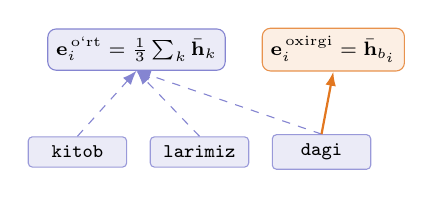
\begin{tikzpicture}[font=\scriptsize]
    \foreach \t/\x [count=\k] in {kitob/0,larimiz/1.55,dagi/3.1}{
      \node[draw=bmain!50,fill=blight,rounded corners=1.5pt,minimum width=1.25cm,font=\scriptsize\ttfamily] (s\k) at (\x,0) {\t};
    }
    \node[box,font=\scriptsize] (em) at (0.75,1.3) {$\vv e_i^{\,\text{o‘rt}}=\tfrac13\sum_k\bar{\vv h}_k$};
    \node[abox,font=\scriptsize] (el) at (3.25,1.3) {$\vv e_i^{\,\text{oxirgi}}=\bar{\vv h}_{b_i}$};
    \foreach \k in {1,2,3} \draw[->,bmain!60,dashed] (s\k.north) -- (em.south);
    \draw[->,accent,thick] (s3.north) -- (el.south);
  \end{tikzpicture}\\[3pt]
  \manba{o‘/g‘ dagi tutuq belgisi (‘) alohida qism so‘zga ajraladi.}
\end{column}
\end{columns}
\yangilik{2}
\end{frame}

%==============================================================================
% 11. YOY VAZNLARI: BI-AFFIN BAHOLASH
%==============================================================================
\begin{frame}{Yoy vaznlari: chuqur bi-affin baholash va ehtimollik modeli}
\begin{columns}[T,onlytextwidth]
\begin{column}{0.6\textwidth}
  \begin{tarif}[5 (chuqur bi-affin baholovchi)]
    \scriptsize $\vv a^{d}_i=\ReLU(\vv W_d\vv r_i+\vv b_d)$, \ $\vv a^{h}_j=\ReLU(\vv W_h\vv r_j+\vv b_h)\in\R^{400}$ (\textbf{tobe}, \textbf{o‘zak});\\[2pt]
    $s_{ij}=[\vv a^{d}_i;1]^{\top}\,\vv U\,[\vv a^{h}_j;1]$,\ \ $\vv U\in\R^{401\times401}$;\ \ yoy belgisi: $s_{ijr}$.
  \end{tarif}
  \begin{lemmauz}[2 (bi-affin forma --- bilinear forma)]
    \scriptsize $\vv U=\begin{bmatrix}\vv U_{11}&\vv u_{12}\\ \vv u_{21}^{\top}&u_{22}\end{bmatrix}$ bo‘lsa, \ $s_{ij}=\vv a^{d\top}_i\vv U_{11}\vv a^{h}_j+\vv u_{21}^{\top}\vv a^{h}_j+c_i$, \ $c_i=\vv a^{d\top}_i\vv u_{12}+u_{22}$.\\[1pt]
    softmax siljishga invariant $\Rightarrow$ $c_i$ ta’sir qilmaydi; $\vv u_{21}^{\top}\vv a^{h}_j$ --- $j$ ning \textbf{o‘zak bo‘lish} aprior bahosi.
  \end{lemmauz}
  \begin{block}{Vazn matritsasi $W$ (yoy yo‘nalishi va Koshi yadrosi bilan)}
    \scriptsize $\tilde s_{ij}=s_{ij}+\log\sigma\big(\lambda_{ij}\sgn(j-i)\big)-\log\big(1+\tfrac12(|j-i|-\delta_{ij})^{2}\big)$;\\[1pt]
    $w_{ji}=\log\softmax_j(\tilde s_{ij})=\log P_\theta(h_i=j\mid x)$,\ \ $P_\theta(r_i=r\mid x,h_i=j)=\softmax_r\,(s_{ijr})$.
  \end{block}
\end{column}
\begin{column}{0.37\textwidth}
  \centering
  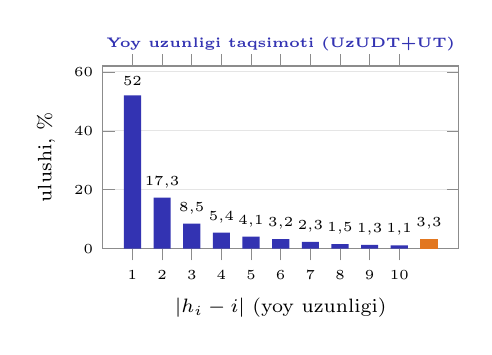
\begin{tikzpicture}
  \begin{axis}[
      width=6.1cm,height=3.9cm,
      ybar,bar width=6.2pt,
      ymin=0,ymax=62,
      symbolic x coords={1,2,3,4,5,6,7,8,9,10,>10},
      xtick=data,
      xlabel={$|h_i-i|$ (yoy uzunligi)},ylabel={ulushi, \%},
      ymajorgrids,
      nodes near coords,
      every node near coord/.append style={font=\tiny,/pgf/number format/fixed,/pgf/number format/precision=1},
      title={\tiny\bfseries\color{bmain} Yoy uzunligi taqsimoti (UzUDT+UT)},
      title style={yshift=-4pt},
    ]
    \addplot[fill=bmain,draw=none,bar shift=0pt] coordinates {(1,52.0)(2,17.3)(3,8.5)(4,5.4)(5,4.1)(6,3.2)(7,2.3)(8,1.5)(9,1.3)(10,1.1)};
    \addplot[fill=accent,draw=none,bar shift=0pt] coordinates {(>10,3.3)};
  \end{axis}
  \end{tikzpicture}\\[3pt]
  \stattile{2.45cm}{84,6\,\%}{o‘zak uch o‘ngda (SOV)}\hfill
  \stattile{2.45cm}{$\bar d=2{,}72$}{o‘rtacha yoy uzunligi}\\[3pt]
  \manba{Tinish belgilari va ildiz yoylarisiz, 13\,512 yoy. Og‘ir dumli taqsimot yoy uzunligi uchun Koshi tipidagi yadro tanlovini asoslaydi.}
\end{column}
\end{columns}
\yangilik{2}
\end{frame}

%==============================================================================
% 12. IKKI OPTIMALLASHTIRISH MASALASI
%==============================================================================
\section{Sonli usullar}
\begin{frame}{Sonli usullar: ikki xil optimallashtirish masalasi}
  \centering
  \renewcommand{\arraystretch}{1.22}
  \footnotesize
  \begin{tabular}{@{}>{\bfseries\raggedright\arraybackslash}p{3.3cm}>{\raggedright\arraybackslash}p{5.1cm}>{\raggedright\arraybackslash}p{5.1cm}@{}}
    \toprule
    & {\color{bmain}\textbf{(P1) Daraxtni topish (dekodlash)}} & {\color{bmain}\textbf{(P2) Parametrlarni topish (o‘qitish)}}\\
    \midrule
    Noma’lum & daraxt $y\in\mathcal T(x)$ & parametrlar $\theta\in\R^{p}$, \ $p=27{,}6\cdot10^{6}$\\
    Maqsad funksiyasi & $W(y)=\sum_{(j\to i)\in y}w_{ji}\ \to\ \max$ & $\widehat R(\theta)$ --- o‘rtacha yo‘qotish $\to\ \min$\\
    Masala turi & diskret: $|\mathcal T(x)|=n^{\,n-1}$ variant & uzluksiz, qavariq emas, stoxastik\\
    Sonli usul & Chu--Liu--Edmonds (MST) & Adam $\to$ AMSGrad, erta to‘xtatish\\
    \textcolor{accent!85!black}{Nima bo‘yicha yutuq} & \textcolor{accent!85!black}{\textbf{vaqt}: $n^{\,n-1}$ variant $\to$ $O(n^2)$ amal} & \textcolor{accent!85!black}{\textbf{aniqlik}: LAS $24{,}7\,\%\to58{,}2\,\%$}\\
    \textcolor{accent!85!black}{Erishilgan natija} & 11 so‘zli gap: $\approx1{,}7$ sutka $\to$ 0,42 ms & E2.1: 1\,000 qadam, 6,3 daqiqa (GPU)\\
    \bottomrule
  \end{tabular}\\[7pt]
  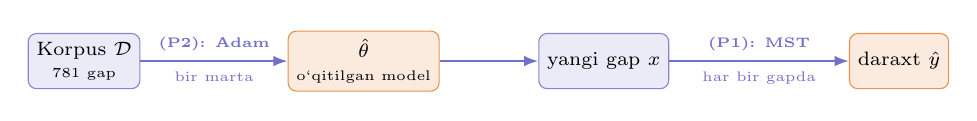
\begin{tikzpicture}[font=\scriptsize,
      nd/.style={rounded corners=3pt,draw=bmain!60,fill=blight,align=center,inner sep=3pt,minimum height=0.7cm}]
    \node[nd] (d) at (0,0) {Korpus $\mathcal D$\\{\tiny 781 gap}};
    \node[nd,fill=accent!15,draw=accent!80] (t) at (3.55,0) {$\hat\theta$\\{\tiny o‘qitilgan model}};
    \node[nd] (x) at (6.6,0) {yangi gap $x$};
    \node[nd,fill=accent!15,draw=accent!80] (y) at (10.35,0) {daraxt $\hat y$};
    \draw[flow] (d) -- node[above,font=\tiny\bfseries] {(P2): Adam} node[below,font=\tiny] {bir marta} (t);
    \draw[flow] (t) -- (x);
    \draw[flow] (x) -- node[above,font=\tiny\bfseries] {(P1): MST} node[below,font=\tiny] {har bir gapda} (y);
  \end{tikzpicture}\\[4pt]
  {\scriptsize\faQuestionCircle\ \textbf{«Optimallashtirish nima bo‘yicha?»} --- (P1) da \textbf{hisoblash vaqti} bo‘yicha (eksponensial $\to$ kvadratik), (P2) da \textbf{yo‘qotish funksiyasi}, ya’ni aniqlik bo‘yicha.}
\yangilik{3, 4}
\end{frame}

%==============================================================================
% 13. SONLI USUL (1): MST
%==============================================================================
\begin{frame}{Sonli usul (1): maksimal vaznli qamrovchi daraxt --- Chu--Liu--Edmonds algoritmi}
\begin{columns}[T,onlytextwidth]
\begin{column}{0.56\textwidth}
  \begin{teorema}[1 (Chu--Liu--Edmonds) va algoritm]
    \scriptsize $G_x$ vaznli to‘liq yo‘naltirilgan graf, $w_{ji}=\log P_\theta(h_i=j\mid x)$ bo‘lsin. Model yoylar bo‘yicha faktorlanganda (P) ning yechimi --- \textbf{maksimal vaznli yo‘naltirilgan qamrovchi daraxt}; uni Chu--Liu--Edmonds algoritmi \textbf{aniq} topadi:\\[3pt]
    \textbf{1)} har bir $i$ uchun eng og‘ir kiruvchi yoy: $h_i=\argmax_j w_{ji}$; \ \textbf{2)} sikl bo‘lmasa --- yechim optimal; \ \textbf{3)} sikl $C$ bitta uchga qisqartiriladi, $w'_{j\to C}=\max_{i\in C}\big(w_{ji}-w_{h_i i}\big)$, masala qayta yechiladi; \ \textbf{4)} $\deg^+(0)>1$ bo‘lsa, nomzod ildizlar bo‘yicha qayta yechiladi.
  \end{teorema}
  \begin{menblock}
    \scriptsize \textbf{1.} Tahlilni maksimal vaznli qamrovchi daraxt masalasiga keltirdim.\\
    \textbf{2.} O‘zgartirgan modelimda daraxtni shu algoritm bilan \textbf{aniq} topdim.\\
    \textbf{3.} Tekshirdim: $n\le7$ da 1\,560 masalada to‘liq saralash bilan \textbf{100\,\%} mos.
  \end{menblock}
\end{column}
\begin{column}{0.41\textwidth}
  \centering
  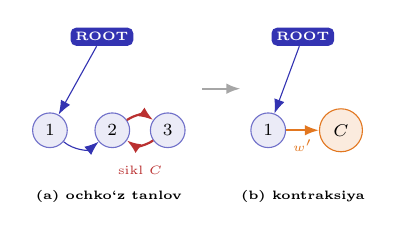
\begin{tikzpicture}[scale=0.88,transform shape,font=\scriptsize,
      nd/.style={circle,draw=bmain!70,fill=blight,inner sep=1.2pt,minimum size=0.5cm},
      rt/.style={rounded corners=2pt,fill=bmain,text=white,inner sep=2pt,font=\tiny\bfseries}]
    % (a) ochko‘z tanlov --- sikl
    \node[rt] (r) at (0,1.35) {ROOT};
    \node[nd] (a) at (-0.75,0) {1}; \node[nd] (b) at (0.15,0) {2}; \node[nd] (c) at (0.95,0) {3};
    \draw[->,bmain] (r) -- (a);
    \draw[->,badred,thick] (b) to[bend left=35] (c);
    \draw[->,badred,thick] (c) to[bend left=35] (b);
    \draw[->,bmain] (a) to[bend right=40] (b);
    \node[font=\tiny,text=badred] at (0.55,-0.58) {sikl $C$};
    \node[font=\tiny\bfseries] at (0.1,-0.95) {(a) ochko‘z tanlov};
    % (b) kontraksiya
    \node[rt] (r2) at (2.9,1.35) {ROOT};
    \node[nd] (a2) at (2.4,0) {1};
    \node[nd,draw=accent,fill=accent!15,minimum size=0.62cm] (C) at (3.45,0) {$C$};
    \draw[->,bmain] (r2) -- (a2);
    \draw[->,accent,thick] (a2) -- node[below,font=\tiny]{$w'$} (C);
    \node[font=\tiny\bfseries] at (2.9,-0.95) {(b) kontraksiya};
    \draw[->,black!35,thick] (1.45,0.6) -- (2.0,0.6);
  \end{tikzpicture}\\[2pt]
  \begin{block}{Murakkablik --- vaqt bo‘yicha}
    \scriptsize To‘liq saralash: $n^{\,n-1}$ daraxt $\times\,O(n)=O(n^{\,n})$ --- \textbf{eksponensial}.\\
    CLE: bitta iteratsiya $O(n^2)$ ($W$ ning har bir elementi bir marta ko‘riladi), iteratsiyalar o‘rtacha 1--2 $\Rightarrow$ \textbf{$O(n^2)$}.
  \end{block}
  \raggedright{\tiny\color{black!65}\textbf{9,2\,\%} gaplar noproyektiv (109 / 1\,184): proyektiv usullar ($O(n^3)$ dinamik dasturlash) ularni ifodalay olmaydi, MST ifodalaydi.\par}
\end{column}
\end{columns}
\yangilik{3}
\end{frame}

%==============================================================================
% 14. HISOBLASH TAJRIBASI: VAQT
%==============================================================================
\begin{frame}{Hisoblash tajribasi: $n^{\,n-1}$ dan $O(n^2)$ ga --- vaqt bo‘yicha yutuq}
\begin{columns}[T,onlytextwidth]
\begin{column}{0.53\textwidth}
  \centering
  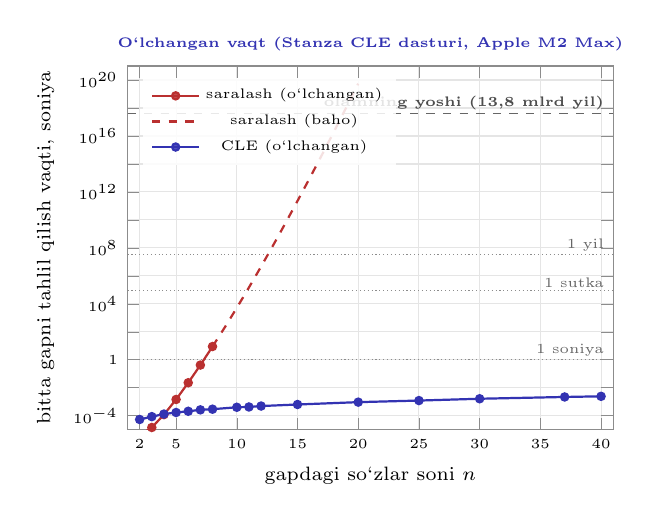
\begin{tikzpicture}
  \begin{axis}[
      width=7.75cm,height=6.2cm,
      ymode=log,
      xmin=1,xmax=41,ymin=1e-5,ymax=1e21,
      xtick={2,5,10,15,20,25,30,35,40},
      ytick={1e-4,1e-2,1e0,1e2,1e4,1e6,1e8,1e10,1e12,1e14,1e16,1e18,1e20},
      yticklabels={$10^{-4}$,,$1$,,$10^{4}$,,$10^{8}$,,$10^{12}$,,$10^{16}$,,$10^{20}$},
      xlabel={gapdagi so‘zlar soni $n$},ylabel={bitta gapni tahlil qilish vaqti, soniya},
      xmajorgrids,ymajorgrids,
      legend style={at={(0.03,0.97)},anchor=north west,font=\tiny},
      title={\tiny\bfseries\color{bmain} O‘lchangan vaqt (Stanza CLE dasturi, Apple M2 Max)},
      title style={yshift=-4pt},
    ]
    % mos yozuv chiziqlari
    \addplot[black!45,densely dotted,forget plot] coordinates {(1,1)(41,1)};
    \addplot[black!45,densely dotted,forget plot] coordinates {(1,86400)(41,86400)};
    \addplot[black!45,densely dotted,forget plot] coordinates {(1,3.156e7)(41,3.156e7)};
    \addplot[black!60,dashed,forget plot] coordinates {(1,4.355e17)(41,4.355e17)};
    \node[font=\tiny,text=black!60,anchor=south east,inner sep=1pt] at (axis cs:40.5,1) {1 soniya};
    \node[font=\tiny,text=black!60,anchor=south east,inner sep=1pt] at (axis cs:40.5,86400) {1 sutka};
    \node[font=\tiny,text=black!60,anchor=south east,inner sep=1pt] at (axis cs:40.5,3.156e7) {1 yil};
    \node[font=\tiny\bfseries,text=black!70,anchor=south east,inner sep=1pt] at (axis cs:40.5,4.355e17) {olamning yoshi (13,8 mlrd yil)};
    % to‘liq saralash: o‘lchangan va baholangan
    \addplot[badred,thick,mark=*,mark size=1.3pt] coordinates {(2,4.067e-06)(3,1.441e-05)(4,1.203e-04)(5,1.454e-03)(6,2.281e-02)(7,4.186e-01)(8,8.857e+00)};
    \addplot[badred,thick,dashed] coordinates {(8,8.857e+00)(9,2.007e+02)(10,5.181e+03)(11,1.478e+05)(12,4.619e+06)(13,1.569e+08)(14,5.757e+09)(15,2.269e+11)(16,9.557e+12)(17,4.286e+14)(18,2.038e+16)(19,1.025e+18)(20,5.432e+19)};
    % CLE: o‘lchangan
    \addplot[bmain,thick,mark=*,mark size=1.3pt] coordinates {(2,5.380e-05)(3,8.600e-05)(4,1.316e-04)(5,1.700e-04)(6,2.080e-04)(7,2.635e-04)(8,2.932e-04)(10,4.017e-04)(11,4.227e-04)(12,4.918e-04)(15,6.340e-04)(20,9.348e-04)(25,1.213e-03)(30,1.633e-03)(37,2.191e-03)(40,2.439e-03)};
    \legend{saralash (o‘lchangan),saralash (baho),CLE (o‘lchangan)}
  \end{axis}
  \end{tikzpicture}
\end{column}
\begin{column}{0.44\textwidth}
  \centering
  \renewcommand{\arraystretch}{1.1}\setlength{\tabcolsep}{3.2pt}
  \scriptsize
  \begin{tabular}{@{}rrrr@{}}
    \toprule
    $n$ & $n^{\,n-1}$ & \textbf{To‘liq saralash} & \textbf{CLE}\\
    \midrule
    5 & 625 & 1,5 ms & 0,17 ms\\
    8 & $2{,}1\cdot10^{6}$ & 8,9 s & 0,29 ms\\
    \textbf{11} & $2{,}6\cdot10^{10}$ & $\approx$\,1,7 sutka$^{*}$ & \textbf{0,42 ms}\\
    20 & $5{,}2\cdot10^{24}$ & $\approx$\,$1{,}7\cdot10^{12}$ yil$^{*}$ & 0,93 ms\\
    37 & $2{,}9\cdot10^{56}$ & $\approx$\,$1{,}7\cdot10^{44}$ yil$^{*}$ & 2,2 ms\\
    \bottomrule
  \end{tabular}\\[1pt]
  \manba{$^{*}$ o‘lchangan tezlik bo‘yicha baho (0,52 mks / variant); 11 --- o‘rtacha, 37 --- eng uzun test gapi. Vaznlar tasodifiy (sikllar ko‘p --- og‘ir holat).}\vspace{4pt}
  \mytile{5.9cm}{$\approx3{,}5\cdot10^{8}$ marta tez}{o‘rtacha (11 so‘zli) gapda: 1,7 sutka $\to$ 0,42 ms}\\[3pt]
  \begin{block}{Tajriba natijalari}
    \scriptsize \textbf{1.} 19 so‘zli gapni saralash \textbf{olamning yoshidan} uzoq.\\
    \textbf{2.} Test to‘plami (198 gap): CLE --- jami \textbf{0,09 s}.\\
    \textbf{3.} $n=20\ldots150$: \ $t_{\mathrm{CLE}}\propto n^{1{,}56}$ \ ($n^2$ dan sekin).
  \end{block}
\end{column}
\end{columns}
\yangilik{3}
\end{frame}

%==============================================================================
% 15. SONLI USUL (2): ADAM
%==============================================================================
\begin{frame}{Sonli usul (2): parametrlarni baholash --- Adam usuli bilan o‘qitish}
\begin{columns}[T,onlytextwidth]
\begin{column}{0.53\textwidth}
  \begin{block}{Masala va Adam iteratsiyasi}
    \scriptsize $\hat\theta=\argmin_{\theta\in\R^{p}}\widehat R(\theta)$, \ $p=27{,}6$ mln; \ $\widehat R=\lambda\widehat R_{\mathrm{UzUDT}}+(1-\lambda)\widehat R_{\mathrm{UT}}$, $\lambda=\tfrac{451}{781}\approx0{,}58$ ($\mathcal L$ --- bir so‘zga o‘rtacha manfiy log-ehtimollik).\\[3pt]
    $\vv g_t=\nabla_\theta\mathcal L_{B_t}(\theta_{t-1})$, \ $\|\vv g_t\|_2\le1$;\ \ $\vv m_t=\beta_1\vv m_{t-1}+(1-\beta_1)\vv g_t$,\ \ $\vv v_t=\beta_2\vv v_{t-1}+(1-\beta_2)\vv g_t^{2}$;\\[1pt]
    $\theta_t=\theta_{t-1}-\alpha\,\hat{\vv m}_t/\big(\sqrt{\hat{\vv v}_t}+\varepsilon\big)$, \ $\hat{\vv m}_t=\vv m_t/(1-\beta_1^{t})$, \ $\hat{\vv v}_t=\vv v_t/(1-\beta_2^{t})$;\\[1pt]
    $\alpha=3\cdot10^{-3}$, $\beta_1=0{,}9$, $\beta_2=0{,}95$, $\varepsilon=10^{-6}$; \ partiya $\le5\,000$ so‘z (UzUDT: 1 davr = 2 qadam).
  \end{block}
\end{column}
\begin{column}{0.44\textwidth}
  \centering
  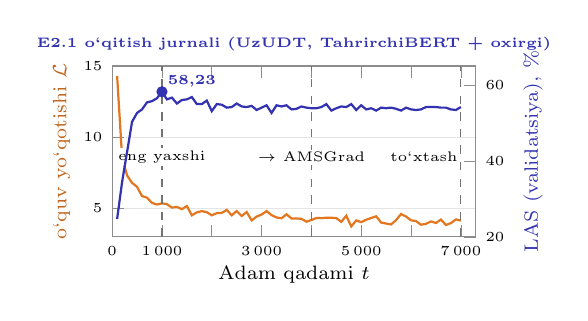
\begin{tikzpicture}
  \begin{axis}[
      width=6.2cm,height=3.75cm,
      xmin=0,xmax=7300,ymin=3,ymax=15,
      axis y line*=left,
      xtick={0,1000,2000,3000,4000,5000,6000,7000},
      xticklabels={0,1\,000,,3\,000,,5\,000,,7\,000},
      scaled x ticks=false,
      xlabel={Adam qadami $t$},
      xlabel style={yshift=3pt},
      ylabel={\color{accent!85!black}o‘quv yo‘qotishi $\mathcal L$},
      ylabel style={yshift=-2pt},
      ymajorgrids,
      title={\tiny\bfseries\color{bmain} E2.1 o‘qitish jurnali (UzUDT, TahrirchiBERT + oxirgi)},
      title style={yshift=-4pt},
    ]
    \addplot[accent,thick] coordinates {(100,14.29)(200,8.57)(300,7.31)(400,6.79)(500,6.51)(600,5.86)(700,5.75)(800,5.38)(900,5.27)(1000,5.35)(1100,5.29)(1200,5.05)(1300,5.10)(1400,4.94)(1500,5.16)(1600,4.51)(1700,4.72)(1800,4.80)(1900,4.73)(2000,4.51)(2100,4.66)(2200,4.68)(2300,4.89)(2400,4.51)(2500,4.81)(2600,4.46)(2700,4.74)(2800,4.15)(2900,4.42)(3000,4.56)(3100,4.81)(3200,4.52)(3300,4.36)(3400,4.30)(3500,4.58)(3600,4.29)(3700,4.29)(3800,4.26)(3900,4.06)(4000,4.18)(4100,4.32)(4200,4.31)(4300,4.34)(4400,4.34)(4500,4.31)(4600,4.05)(4700,4.48)(4800,3.73)(4900,4.15)(5000,4.03)(5100,4.20)(5200,4.32)(5300,4.44)(5400,4.00)(5500,3.93)(5600,3.87)(5700,4.17)(5800,4.60)(5900,4.42)(6000,4.16)(6100,4.10)(6200,3.85)(6300,3.91)(6400,4.08)(6500,3.97)(6600,4.21)(6700,3.83)(6800,3.96)(6900,4.22)(7000,4.14)};
    \draw[black!55,dashed] (axis cs:1000,3) -- (axis cs:1000,15);
    \draw[black!55,dashed] (axis cs:4000,3) -- (axis cs:4000,15);
    \draw[black!55,dashed] (axis cs:7000,3) -- (axis cs:7000,15);
    \node[font=\tiny,fill=white,inner sep=1pt] at (axis cs:1000,8.6) {eng yaxshi};
    \node[font=\tiny,fill=white,inner sep=1pt] at (axis cs:4000,8.6) {$\to$ AMSGrad};
    \node[font=\tiny,fill=white,inner sep=1pt,anchor=east] at (axis cs:7000,8.6) {to‘xtash};
  \end{axis}
  \begin{axis}[
      width=6.2cm,height=3.75cm,
      xmin=0,xmax=7300,ymin=20,ymax=65,
      axis y line*=right,axis x line=none,
      ylabel={\color{bmain}LAS (validatsiya), \%},
      ylabel near ticks,yticklabel pos=right,
    ]
    \addplot[bmain,thick] coordinates {(100,24.69)(200,34.47)(300,42.39)(400,50.31)(500,52.64)(600,53.57)(700,55.43)(800,55.75)(900,56.52)(1000,58.23)(1100,56.21)(1200,56.68)(1300,55.12)(1400,56.06)(1500,56.21)(1600,56.83)(1700,54.97)(1800,54.97)(1900,55.90)(2000,53.11)(2100,54.97)(2200,54.81)(2300,54.04)(2400,54.19)(2500,55.12)(2600,54.35)(2700,54.19)(2800,54.50)(2900,53.42)(3000,54.04)(3100,54.66)(3200,52.64)(3300,54.66)(3400,54.35)(3500,54.66)(3600,53.57)(3700,53.73)(3800,54.35)(3900,54.04)(4000,53.88)(4100,53.88)(4200,54.19)(4300,54.97)(4400,53.26)(4500,53.88)(4600,54.35)(4700,54.19)(4800,54.97)(4900,53.42)(5000,54.66)(5100,53.57)(5200,53.88)(5300,53.26)(5400,54.04)(5500,53.88)(5600,54.04)(5700,53.73)(5800,53.26)(5900,54.04)(6000,53.57)(6100,53.42)(6200,53.57)(6300,54.19)(6400,54.19)(6500,54.19)(6600,54.04)(6700,54.04)(6800,53.57)(6900,53.42)(7000,54.19)};
    \addplot[only marks,mark=*,mark size=1.8pt,bmain] coordinates {(1000,58.23)};
    \node[font=\tiny\bfseries,text=bmain,anchor=south west,inner sep=1pt] at (axis cs:1050,58.6) {58,23};
  \end{axis}
  \end{tikzpicture}
\end{column}
\end{columns}
\begin{columns}[T,onlytextwidth]
\begin{column}{0.53\textwidth}
  \begin{menblock}
    \scriptsize \textbf{1.} Ikki korpus uchun maqsad funksiyasini tuzdim.\\
    \textbf{2.} BERT ni muzlatdim: $137\to27{,}6$ mln parametr ($\approx$5 marta kam).\\
    \textbf{3.} To‘xtatish: 3\,000 qadam yaxshilanmasa --- AMSGrad, yana 3\,000 --- to‘xtash.\\
    \textbf{4.} Jurnallashtirib, 5 tajribada yaqinlashishni tahlil qildim.
  \end{menblock}
\end{column}
\begin{column}{0.44\textwidth}
  \begin{block}{Natija (E2.1)}
    \scriptsize Yo‘qotish $14{,}29\to5{,}35$ ($-63\,\%$), LAS $24{,}7\to\mathbf{58{,}2}\,\%$ --- \textbf{1\,000 qadamda}, 375 s (RTX A6000). Keyin LAS $\approx54\,\%$ ga tushadi (haddan tashqari moslashish) $\Rightarrow$ eng yaxshi nuqta saqlanadi. 5 tajribada eng yaxshi qadam: 800--1\,300.
  \end{block}
\end{column}
\end{columns}
\yangilik{4}
\end{frame}

%==============================================================================
% 16. MA’LUMOTLAR VA TAJRIBA DIZAYNI
%==============================================================================
\section{Tajribalar}
\begin{frame}{Ma’lumotlar va tajriba dizayni}
\begin{columns}[T,onlytextwidth]
\begin{column}{0.53\textwidth}
  \renewcommand{\arraystretch}{1.1}
  \scriptsize
  \setlength{\tabcolsep}{4pt}
  \begin{tabular}{@{}lll@{}}
    \toprule
    & \textbf{UzUDT} (men yaratgan) & \textbf{UT}\\
    \midrule
    Janr & badiiy, ta’limiy & yangilik, badiiy\\
    Gap / token & 684 / 7\,582 & 500 / 5\,930\\
    Annotatsiya & qo‘lda, 6 annotator & yarim avtomatik\\
    Kelishuv ($\kappa$, \%) & lemma 95,2; UPOS 93,7 & ---\\
    UD validatsiyasi & \textcolor{okgreen}{\faCheck}\ o‘tgan & \textcolor{badred}{\faTimes}\ 92 ogohl.\\
    Noproyektiv daraxtlar & 11,0\,\% & 6,8\,\%\\
    Bog‘lanish turlari & 38 & 33 \ (jami 39)\\
    \bottomrule
  \end{tabular}\\[6pt]
  {\color{bmain}\bfseries\small Tajriba rejasi: $3\times2$ faktorli dizayn}\\[3pt]
  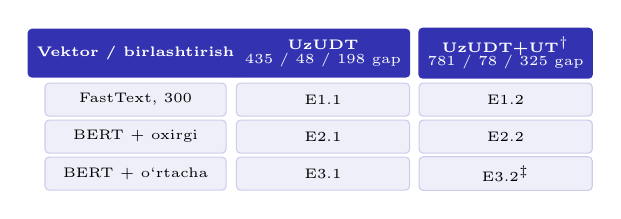
\begin{tikzpicture}[font=\tiny,
      hd/.style={fill=bmain,text=white,rounded corners=1.5pt,minimum height=0.48cm,font=\tiny\bfseries,align=center},
      cl/.style={fill=bmain!8,draw=bmain!25,rounded corners=1.5pt,minimum width=1.9cm,minimum height=0.42cm,align=center}]
    \node[hd,minimum width=2.3cm,minimum height=0.62cm] at (0,0) {Vektor / birlashtirish};
    \node[hd,minimum width=2.2cm,minimum height=0.62cm] at (2.38,0) {UzUDT\\[-1pt]{\tiny\mdseries 435 / 48 / 198 gap}};
    \node[hd,minimum width=2.2cm,minimum height=0.62cm] at (4.7,0) {UzUDT+UT$^\dagger$\\[-1pt]{\tiny\mdseries 781 / 78 / 325 gap}};
    \foreach \t/\a/\b [count=\i] in {{FastText, 300}/E1.1/E1.2, {BERT + oxirgi}/E2.1/E2.2, {BERT + o‘rtacha}/E3.1/E3.2$^\ddagger$}{
      \node[cl,minimum width=2.3cm] at (0,-0.12-0.47*\i) {\t};
      \node[cl,minimum width=2.2cm] at (2.38,-0.12-0.47*\i) {\a};
      \node[cl,minimum width=2.2cm] at (4.7,-0.12-0.47*\i) {\b};
    }
  \end{tikzpicture}\\[1pt]
  \manba{$^\dagger$ bu sharoitda parserga oltin UPOS/XPOS/UFeats berilgan. \ $^\ddagger$ E3.2 jurnali repozitoriyda yo‘q.}
\end{column}
\begin{column}{0.44\textwidth}
  \centering
  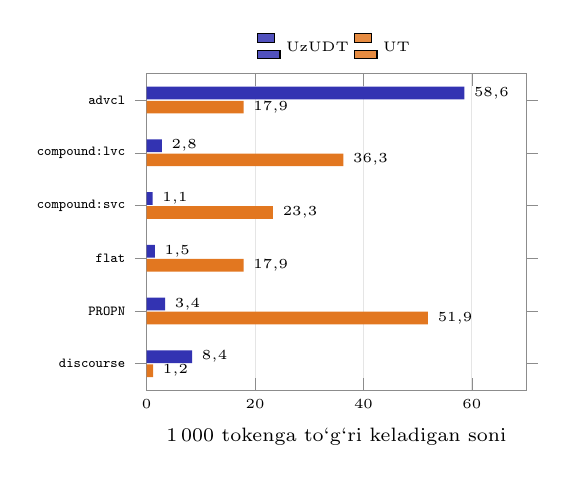
\begin{tikzpicture}
  \begin{axis}[
      width=6.4cm,height=5.6cm,
      xbar=0.5pt,bar width=4.6pt,
      xmin=0,xmax=70,
      symbolic y coords={discourse,PROPN,flat,svc,lvc,advcl},
      ytick=data,
      yticklabels={discourse,PROPN,flat,compound:svc,compound:lvc,advcl},
      yticklabel style={font=\tiny\ttfamily},
      xlabel={1\,000 tokenga to‘g‘ri keladigan soni},
      xmajorgrids,
      nodes near coords,
      every node near coord/.append style={font=\tiny,/pgf/number format/fixed,/pgf/number format/precision=1},
      legend style={at={(0.5,1.02)},anchor=south,legend columns=2},
      reverse legend,
    ]
    \addplot[fill=accent,draw=none] coordinates {(1.2,discourse)(51.9,PROPN)(17.9,flat)(23.3,svc)(36.3,lvc)(17.9,advcl)};
    \addplot[fill=bmain,draw=none] coordinates {(8.4,discourse)(3.4,PROPN)(1.5,flat)(1.1,svc)(2.8,lvc)(58.6,advcl)};
    \legend{UT,UzUDT}
  \end{axis}
  \end{tikzpicture}\\[-2pt]
  \manba{Korpuslar bir-birini to‘ldiradi. Manba: data/udbase/*.conllu.}
\end{column}
\end{columns}
\yangilik{1}
\end{frame}

%==============================================================================
% 17. NATIJALAR
%==============================================================================
\begin{frame}{Natijalar: validatsiya to‘plami, eng yaxshi nazorat nuqtasi}
\begin{columns}[T,onlytextwidth]
\begin{column}{0.53\textwidth}
  \renewcommand{\arraystretch}{1.08}
  \scriptsize
  \setlength{\tabcolsep}{4pt}
  \begin{tabular}{@{}llrrrr@{}}
    \toprule
    & & \multicolumn{2}{c}{\textbf{Teglash}} & \multicolumn{2}{c}{\textbf{Sintaktik tahlil}}\\
    \cmidrule(lr){3-4}\cmidrule(l){5-6}
    \textbf{Tajriba} & \textbf{Vektorlar} & UPOS & UFeats & UAS & LAS\\
    \midrule
    \multicolumn{6}{@{}l}{\tiny\itshape A. UzUDT; parserga bashorat qilingan teglar (48 gap, 644 token)}\\
    E1.1 & FastText & 79,19 & 66,61 & 71,58 & 55,28\\
    E2.1 & BERT + oxirgi & \textbf{83,54} & \textbf{68,17} & \textbf{73,91} & \textbf{58,23}\\
    E3.1 & BERT + o‘rtacha & 83,39 & 65,84 & 71,58 & 55,90\\
    \midrule
    \multicolumn{6}{@{}l}{\tiny\itshape B. UzUDT+UT; parserga oltin teglar$^\dagger$ (78 gap, 851 token)}\\
    E1.2 & FastText & 83,78 & 70,98 & 70,51 & 62,87\\
    E2.2 & BERT + oxirgi & \textbf{87,19} & \textbf{73,21} & \textbf{72,39} & \textbf{63,81}\\
    \bottomrule
  \end{tabular}\\[5pt]
  \begin{block}{Xulosalar}
    \scriptsize \textbf{1.} Sintaktik tahlilda «oxirgi qism so‘z» operatori o‘rtacha qiymatdan \textbf{ishonchli} yaxshi.\\
    \textbf{2.} TahrirchiBERT teglashni yaxshilaydi: UPOS $+3{,}4\ldots+4{,}4$ punkt.\\
    \textbf{3.} Oltin morfologiya berilganda BERT ning sintaktik ustunligi ahamiyatsiz.
  \end{block}
\end{column}
\begin{column}{0.44\textwidth}
  \centering
  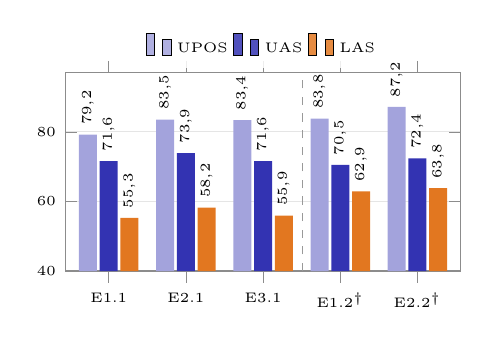
\begin{tikzpicture}
  \begin{axis}[
      width=6.6cm,height=4.1cm,
      ybar=1pt,bar width=6.5pt,
      ymin=40,ymax=97,
      symbolic x coords={E1.1,E2.1,E3.1,E1.2,E2.2},
      xtick=data,
      xticklabels={E1.1,E2.1,E3.1,E1.2$^\dagger$,E2.2$^\dagger$},
      ymajorgrids,
      nodes near coords,
      every node near coord/.append style={font=\tiny,rotate=90,anchor=west,/pgf/number format/fixed,/pgf/number format/precision=1},
      legend style={at={(0.5,1.02)},anchor=south,legend columns=3},
      enlarge x limits=0.14,
    ]
    \addplot[fill=bmain!45,draw=none] coordinates {(E1.1,79.19)(E2.1,83.54)(E3.1,83.39)(E1.2,83.78)(E2.2,87.19)};
    \addplot[fill=bmain,draw=none] coordinates {(E1.1,71.58)(E2.1,73.91)(E3.1,71.58)(E1.2,70.51)(E2.2,72.39)};
    \addplot[fill=accent,draw=none] coordinates {(E1.1,55.28)(E2.1,58.23)(E3.1,55.90)(E1.2,62.87)(E2.2,63.81)};
    \legend{UPOS,UAS,LAS}
    \draw[black!40,dashed] ([xshift=0.5cm]axis cs:E3.1,40) -- ([xshift=0.5cm]axis cs:E3.1,97);
  \end{axis}
  \end{tikzpicture}\\[1pt]
  \begin{block}{Juftlashgan bootstrap, $B=10^4$}
    \scriptsize $\Delta^{*}_b=\mathrm{LAS}_A(S^{*}_b)-\mathrm{LAS}_B(S^{*}_b)$;\ 95\,\% IO $=\big[\Delta^{*}_{(0{,}025)};\Delta^{*}_{(0{,}975)}\big]$\\[1pt]
    oxirgi -- o‘rt.: \ $+2{,}64$\ $[+0{,}97;+4{,}12]$, $p\approx0{,}002$ \textcolor{okgreen}{\faCheck}\\
    BERT -- FT (A): \ $+2{,}95$\ $[0{,}00;+5{,}63]$, $p\approx0{,}03$\\
    BERT -- FT (B): \ $-1{,}29$\ $[-4{,}66;+2{,}23]$ --- ahamiyatsiz
  \end{block}
\end{column}
\end{columns}
\vspace{-2pt}
\manba{$^\dagger$ A va B bevosita taqqoslanmaydi: kiruvchi teglar (bashorat / oltin) va validatsiya to‘plamlari farqli. Bootstrap --- oxirgi qadam bashoratlari bo‘yicha.}
\yangilik{2}
\end{frame}

%==============================================================================
% 18. TEST, TURG‘UNLIK, DEKODLASH
%==============================================================================
\begin{frame}{Test to‘plamida baholash: turg‘unlik va dekodlash usullarini taqqoslash}
\begin{columns}[T,onlytextwidth]
\begin{column}{0.52\textwidth}
  \begin{tarif}[6 (sezgirlik)]
    \scriptsize $\pi$ --- matnni buzuvchi (g‘alayon) operatori, $\rho_\pi$ --- o‘zgargan tokenlar ulushi;\ \ sezgirlik: \ $S_\pi=\mathrm{LAS}(\mathcal D)-\mathrm{LAS}\big(\pi(\mathcal D)\big)$.
  \end{tarif}
  \centering
  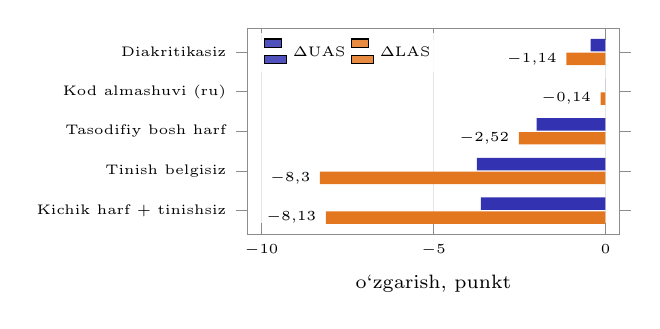
\begin{tikzpicture}
  \begin{axis}[
      width=6.3cm,height=4.2cm,
      xbar=0.5pt,bar width=4.5pt,
      xmin=-10.4,xmax=0.4,
      ymin=0.4,ymax=5.6,
      ytick={1,2,3,4,5},
      yticklabels={Kichik harf + tinishsiz,Tinish belgisiz,Tasodifiy bosh harf,Kod almashuvi (ru),Diakritikasiz},
      yticklabel style={font=\tiny},
      xlabel={o‘zgarish, punkt},
      xmajorgrids,
      legend style={at={(0.02,0.98)},anchor=north west,legend columns=2},
      reverse legend,
    ]
    \addplot[fill=accent,draw=none,nodes near coords,every node near coord/.append style={font=\tiny,anchor=east,/pgf/number format/fixed,/pgf/number format/precision=2}] coordinates {(-8.13,1)(-8.30,2)(-2.52,3)(-0.14,4)(-1.14,5)};
    \addplot[fill=bmain,draw=none] coordinates {(-3.62,1)(-3.74,2)(-2.00,3)(0,4)(-0.43,5)};
    \legend{$\Delta$LAS,$\Delta$UAS}
  \end{axis}
  \end{tikzpicture}\\[-2pt]
  \raggedright\manba{E2.1 modeli, UzUDT test to‘plami (198 gap, 2\,101 token); toza matnda UAS 71,06, LAS 54,07. $\rho_\pi$: diakritika 8,7\,\%, kod almashuvi 0,2\,\%, bosh harf 53,3\,\%, tinish belgisi 19,6\,\%.}
\end{column}
\begin{column}{0.45\textwidth}
  \centering
  {\scriptsize\bfseries\color{bmain} MST va ochko‘z dekodlash (bir xil test)}\\[3pt]
  \renewcommand{\arraystretch}{1.2}
  \scriptsize
  \begin{tabular}{@{}lccc@{}}
    \toprule
    & \textbf{Graf + MST} & \textbf{O‘tish (arc-eager)} & $\Delta$\\
    & {\tiny Stanza, E2.1} & {\tiny spaCy, S1.1} & \\
    \midrule
    UAS & \textbf{71,06} & 67,72 & $+3{,}34$\\
    LAS & \textbf{54,07} & 45,35 & $+8{,}72$\\
    \bottomrule
  \end{tabular}\\[2pt]
  \manba{Ikkalasi ham TahrirchiBERT; spaCy baholovchisi tinish belgilarini hisobga olmaydi.}\vspace{6pt}
  \begin{block}{Talqin}
    \scriptsize \textbf{1.} Global (MST) optimallashtirish ochko‘z ketma-ket qarorlardan \textbf{8,7 punkt} yaxshi: xatolar zanjir bo‘ylab tarqalmaydi.\\
    \textbf{2.} Diakritika yo‘qolishiga turg‘un ($-1{,}1$), kod almashuviga deyarli befarq ($-0{,}1$).\\
    \textbf{3.} Tinish belgilari --- muhim tuzilmaviy signal: ularsiz LAS $8{,}3$ punktga tushadi.
  \end{block}
\end{column}
\end{columns}
\yangilik{3, 4}
\end{frame}

%==============================================================================
% 19. DASTURIY MAJMUA
%==============================================================================
\section{Dasturiy majmua}
\begin{frame}{Dasturiy majmua}
  \centering
  \begin{tikzpicture}[
      col/.style={rounded corners=4pt,fill=bmain,text=white,font=\scriptsize\bfseries,minimum width=3.25cm,minimum height=0.55cm},
      it/.style={rounded corners=2pt,fill=bmain!7,draw=bmain!25,text width=3.05cm,font=\scriptsize,align=left,inner sep=3pt,anchor=north,minimum height=2.3cm}]
    \foreach \x/\h/\b [count=\i] in {
      0/{\faDatabase\ Ma’lumotlar}/{UzUDT (UD v2.17, CC BY-SA 4.0) va UT\\[2pt] CoNLL-U o‘quvchi va birlashtiruvchi\\[2pt] spaCy DocBin konvertori\\[2pt] korpus statistikasi},
      3.65/{\faCogs\ O‘qitish}/{Stanza: BERT kanali va $\Pi$ operatori (\texttt{-{}-bert\_model}, \texttt{-{}-bert\_pooling})\\[2pt] spaCy uchun \texttt{uz} til moduli\\[2pt] CSV / W\&B jurnallari},
      7.3/{\faChartBar\ Baholash}/{CoNLL 2018 metrikalari (UAS, LAS, MLAS, BLEX)\\[2pt] juftlashgan bootstrap\\[2pt] g‘alayon (turg‘unlik) testlari\\[2pt] MST vaqt tajribasi},
      10.95/{\faUpload\ E’lon qilish}/{HuggingFace: \texttt{Sanatbek/uzudt}\\[2pt] GitHub: \texttt{robust-parsing-uzbek}\\[2pt] UD rasmiy repozitoriysi}}{
      \node[col] (h\i) at (\x,0) {\h};
      \node[it] (b\i) at (\x,-0.45) {\b};
    }
    \foreach \i/\j in {1/2,2/3,3/4} \draw[->,very thick,bmain!50] (h\i.east) -- (h\j.west);
  \end{tikzpicture}\\[6pt]
  \begin{columns}[T,onlytextwidth]
  \begin{column}{0.56\textwidth}
    \begin{menblock}[\faCode\ Men Stanza kutubxonasiga kiritgan o‘zgarishlar]
      \scriptsize
      \texttt{depparse/model.py} --- tahlilchiga BERT kanali, ildiz uchun $\vv e_0=\vv 0$\\
      \texttt{common/bert\_embedding.py} --- $\Pi$ operatori: \texttt{last} / \texttt{mean}\\
      \texttt{depparse/data.py}, \texttt{trainer.py} --- xom tokenlar, BERT ni ulash\\
      \texttt{pos/model.py}, \texttt{tagger.py}, \texttt{parser.py} --- teglovchi, CLI, jurnallar\\
      \texttt{common/constant.py} --- \texttt{uz} (o‘zbek tili) kodi
    \end{menblock}
  \end{column}
  \begin{column}{0.41\textwidth}
    \begin{block}{Hajmi va texnik ko‘rsatkichlar}
      \scriptsize Stanza: $\approx$570 qator (20 fayl); spaCy-uz moduli: $\approx$920; baholash skriptlari: $\approx$1\,600 $\Rightarrow$ \textbf{$\approx$3\,100 qator} Python kodi.\\[2pt]
      Python, PyTorch, Stanza, spaCy 3.8; o‘qitish --- NVIDIA RTX A6000.
    \end{block}
  \end{column}
  \end{columns}
\yangilik{4}
\end{frame}

%==============================================================================
% 20. XULOSA
%==============================================================================
\section{Xulosa}
\begin{frame}{Xulosa}
  \scriptsize
  \begin{columns}[T,onlytextwidth]
  \begin{column}{0.495\textwidth}
  \begin{enumerate}\setlength{\itemsep}{3pt}
    \item O‘zbek tilining badiiy va ta’limiy matnlari uchun \textbf{ilk bor} oltin standart UD korpusi \textbf{UzUDT} (684 gap, 7\,582 token) yaratildi va e’lon qilindi.
    \item Sintaktik tahlil \textbf{graflar nazariyasi} tilida qo‘yildi: gap --- vaznli to‘liq yo‘naltirilgan graf, tahlil natijasi --- maksimal vaznli qamrovchi daraxt; daraxtlar soni $n^{\,n-1}$.
    \item Stanza bi-affin tahlilchisi o‘zgartirildi: TahrirchiBERT kanali va $\Pi$ operatori ($\R^{500}\to\R^{1143}$); \textbf{ilk bor} «oxirgi qism so‘z» operatorining ustunligi tasdiqlandi ($+2{,}6$ LAS, $p\approx0{,}002$).
  \end{enumerate}
  \end{column}
  \begin{column}{0.495\textwidth}
  \begin{enumerate}\setcounter{enumi}{3}\setlength{\itemsep}{3pt}
    \item Daraxtni izlash murakkabligi $n^{\,n-1}$ dan \textbf{$O(n^2)$} ga tushirildi: 11 so‘zli gapda $\approx1{,}7$ sutka $\to$ 0,42 ms; MST ochko‘z o‘tish usulidan LAS bo‘yicha \textbf{8,7 punkt} yuqori.
    \item Adam$\to$AMSGrad bilan o‘qitishda 1\,000 qadamda (6,3 daqiqa) LAS $24{,}7\to58{,}2\,\%$; model diakritikaga turg‘un, tinish belgilariga sezgir ($-8{,}3$ LAS).
    \item \textbf{Dasturiy majmua} ($\approx$3\,100 qator Python) yaratildi, korpus va modellar ochiq e’lon qilindi.
  \end{enumerate}
  \end{column}
  \end{columns}
  \vspace{4pt}
  \begin{block}{Kelgusi ishlar}
    \scriptsize Barcha tajribalarni yagona bo‘linma va bashorat qilingan teglar bilan \textbf{test to‘plamida} qayta baholash; ko‘p urug‘li (seed) tajribalar; global normallash (Kirchhoff matritsa-daraxt teoremasi, $Z(x)=\det\widehat{\vv L}$); BERTbek va FastText+BERT birikmasi.
  \end{block}
  \centering
  \stattile{3.15cm}{684 gap}{UzUDT korpusi}\
  \mytile{3.15cm}{$n^{\,n-1}\to O(n^2)$}{daraxtni izlash (vaqt)}\
  \stattile{3.15cm}{$+2{,}6$ LAS}{oxirgi qism so‘z ($p\approx0{,}002$)}\
  \mytile{3.15cm}{58,2 LAS}{1\,000 qadamda (Adam)}
\end{frame}

%==============================================================================
% 21. APROBATSIYA VA NASHRLAR
%==============================================================================
\begin{frame}{Natijalarning aprobatsiyasi va e’lon qilinganligi}
  \setbeamertemplate{enumerate items}[default]
  \scriptsize\urlstyle{same}
  % Manba: bib/*.bib (APA 7); Scopus kvartili --- bib fayl nomidan
  \begin{enumerate}\setlength{\itemsep}{4pt}
    \item Matlatipov, S., Aripov, M., Bobokandov, M., \& Matlatipov, G. (2026). Annotated Universal Dependencies dataset for literary and educational Uzbek texts. \textit{Data in Brief}, \textit{66}, Article 112857. \url{https://doi.org/10.1016/j.dib.2026.112857} \textbf{[Scopus, Q1]}
    \item Matlatipov, S. (2027). Towards robust Uzbek neural dependency parsing: Cross-treebank training. In E.~Cabrio \& E.~Monteiro (Eds.), \textit{Natural language processing and information systems} (pp.~204--218). Springer Nature Switzerland. \url{https://doi.org/10.1007/978-3-032-29532-3_15} \textbf{[Scopus, Q2]}
    \item Matlatipov, S., Ismoilova, M., \& Aripov, M. (2026). Graph-based vs transition-based dependency parsing for Uzbek. In \textit{2026 IEEE 27th International Conference of Young Professionals in Electron Devices and Materials (EDM)} (pp.~1--6). IEEE. \url{https://doi.org/10.1109/EDM69524.2026.11632281} \textbf{[Scopus, Q3]}
    \item Matlatipov, S. G., \& Aripov, M. (2026). UzUDT: Uzbek Universal Dependencies treebank. In S.~Piperidis, N.~Bel, H.~van den Heuvel, N.~Ide, S.~Krek, \& A.~Toral (Eds.), \textit{Proceedings of the Fifteenth Language Resources and Evaluation Conference} (pp.~11642--11649). ELRA Language Resource Association. \url{https://doi.org/10.63317/2uedjqezjxn5} \textbf{[Scopus]}
    \item Matlatipov, S., \& Kurbanova, M. (2026). A gold-standard dependency treebank for the Uzbek language. In \textit{2026 IEEE Ural-Siberian Conference on Biomedical Engineering, Radioelectronics and Information Technology (USBEREIT)} (pp.~1--3). IEEE. \url{https://doi.org/10.1109/USBEREIT70063.2026.11580531} \textbf{[Scopus]}
    \item Matlatipov, S. (2026). Neural morphosyntactic tagging and dependency parsing for Uzbek. In \textit{2026 IEEE Ural-Siberian Conference on Biomedical Engineering, Radioelectronics and Information Technology (USBEREIT)} (pp.~1--4). IEEE. \url{https://doi.org/10.1109/USBEREIT70063.2026.11580890} \textbf{[Scopus]}
  \end{enumerate}
\end{frame}

%==============================================================================
% 22. YAKUN
%==============================================================================
\begin{frame}
  \centering
  \titlebox{0.62\textwidth}{\LARGE\bfseries E’tiboringiz uchun rahmat!}\\[22pt]
  {\small\bfseries Matlatipov Sanatbek}\\[3pt]
  {\footnotesize Mirzo Ulug‘bek nomidagi O‘zbekiston Milliy universiteti}\\[10pt]
  {\footnotesize \faEnvelope\ s.matlatipov@nuu.uz \qquad \faGithub\ SanatbekMatlatipov/robust-parsing-uzbek}
\end{frame}

%==============================================================================
% ZAXIRA SLAYD (savollar uchun): BiLSTM
%==============================================================================
\appendix
\begin{frame}{Zaxira slayd: kontekstni hisobga oluvchi kodlovchi --- highway BiLSTM}
\begin{columns}[T,onlytextwidth]
\begin{column}{0.57\textwidth}
  \begin{block}{Kirish vektori}
    \scriptsize $\vv v_i=\big[\vv e^{w}_i;\ \vv e^{\mathrm{lem}}_i;\ \vv e^{\mathrm{upos}}_i+\vv e^{\mathrm{xpos}}_i;\ \textstyle\sum_k\vv e^{f_k}_i;\ \vv W_c\vv c_i;\ \vv e_i\big]\in\R^{1143}$\\[1pt]
    {\tiny so‘z $75$ + lemma $75$ + teglar $50$ + belgilar $50$ + harf-LSTM $125$ + BERT $768$ \ (FastText variantida $\vv e_i$ o‘rniga $\vv W_p\vv p_i\in\R^{125}$, jami $500$)}
  \end{block}
  \begin{block}{LSTM yacheykasi (S.~Hochreiter, J.~Schmidhuber, 1997)}
    \scriptsize
    $\begin{pmatrix}\vv i_t\\ \vv f_t\\ \vv o_t\\ \vv g_t\end{pmatrix}=\begin{pmatrix}\sigma\\ \sigma\\ \sigma\\ \tanh\end{pmatrix}\!\left(\vv W\begin{bmatrix}\vv v_t\\ \vv h_{t-1}\end{bmatrix}+\vv b\right)$,\qquad
    $\begin{aligned}\vv c_t&=\vv f_t\odot\vv c_{t-1}+\vv i_t\odot\vv g_t,\\ \vv h_t&=\vv o_t\odot\tanh(\vv c_t).\end{aligned}$
  \end{block}
  \begin{block}{Ikki yo‘nalish va highway bog‘lanish, \ $\ell=1,2,3$}
    \scriptsize $\vv z^{(\ell)}_t=\big[\overrightarrow{\vv h}^{(\ell)}_t;\overleftarrow{\vv h}^{(\ell)}_t\big]+\sigma\big(\vv G^{(\ell)}\vv z^{(\ell-1)}_t\big)\odot\tanh\big(\vv W_H^{(\ell)}\vv z^{(\ell-1)}_t\big)$,\quad $\vv r_i=\vv z^{(3)}_i\in\R^{800}$
  \end{block}
\end{column}
\begin{column}{0.4\textwidth}
  \centering
  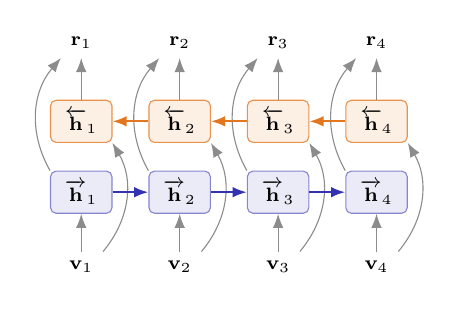
\begin{tikzpicture}[font=\scriptsize,
      cell/.style={rounded corners=2pt,draw=bmain!60,fill=blight,minimum width=0.78cm,minimum height=0.5cm},
      bcell/.style={rounded corners=2pt,draw=accent!80,fill=accent!12,minimum width=0.78cm,minimum height=0.5cm}]
    \foreach \i in {1,...,4}{
      \node (v\i) at (1.25*\i,0) {$\vv v_{\i}$};
      \node[cell] (f\i) at (1.25*\i,0.95) {$\overrightarrow{\vv h}_{\i}$};
      \node[bcell] (b\i) at (1.25*\i,1.85) {$\overleftarrow{\vv h}_{\i}$};
      \node (r\i) at (1.25*\i,2.85) {$\vv r_{\i}$};
      \draw[->,black!45] (v\i) -- (f\i);
      \draw[->,black!45] (v\i.north east) to[bend right=35] (b\i.south east);
      \draw[->,black!45] (b\i) -- (r\i);
      \draw[->,black!45] (f\i.north west) to[bend left=35] (r\i.south west);
    }
    \foreach \i/\j in {1/2,2/3,3/4}{
      \draw[->,bmain,thick] (f\i) -- (f\j);
      \draw[->,accent,thick] (b\j) -- (b\i);
    }
  \end{tikzpicture}\\[4pt]
  \begin{block}{Gradient oqimi}
    \scriptsize To‘g‘ridan-to‘g‘ri yo‘l bo‘yicha $\dfrac{\partial\vv c_t}{\partial\vv c_{t-1}}=\operatorname{diag}(\vv f_t)$: unutish darvozasi uzoq bog‘lanishlarda gradientning so‘nishini yumshatadi.
  \end{block}
  {\tiny\color{black!60} Teglovchi: 2 qatlam, $2\times200$; \ parser: 3 qatlam, $2\times400$.}
\end{column}
\end{columns}
\end{frame}

\end{document}
